\documentclass[10pt,a4paper,twoside]{llncs}
\usepackage[left=3cm,right=3cm,top=2.5cm,bottom=2.5cm]{geometry}
\setcounter{secnumdepth}{3}%to set numbering over subsubsections
\usepackage[utf8]{inputenc}
\usepackage{color}
\usepackage{amsmath,amsfonts,amssymb}
\usepackage{graphicx,float}
\usepackage{algorithmic,algorithm}
\usepackage{tikz}
\usetikzlibrary{matrix}
\usetikzlibrary{matrix,arrows,shapes}%,decorations.pathmorphing,snakes

\pagestyle{headings}%page numbers

%%%%%%%%%%%%%%%%%%%%%%%%%%% VERSIONES %%%%%%%%%%%%%%%%%%%%%%%%%%%%%%%%%%%%%%%%%
%%%% This file is generated by Makefile.
%%% Do not edit this file!
%%%
	\gdef\GITAbrHash{74b8017}	\gdef\GITAuthorDate{Sat Sep 15 21:59:40 2012 +0200}	\gdef\GITAuthorName{srgblnch}
%\newcommand{\version}{git: \GITAuthorDate \; (revision~\GITAbrHash)}

\usepackage{gitinfo}
\newcommand{\version}{github.Papers: \gitCommitterDate\;(revision \gitAbbrevHash) }
\newcommand{\todo}[1]{\texttt{\color{red}TODO:} ``\emph{#1}''}
\newcommand{\fixme}[1]{\texttt{\color{red}FIXME:} ``\emph{#1}''}
%%%%%%%%%%%%%%%%%%%%%%%%%%%%%%%%%%%%%%%%%%%%%%%%%%%%%%%%%%%%%%%%%%%%%%%%%%%%%%%

\title{Generalised Rijndael}
\author{Sergi Blanch-Torn\'e\inst{1}, Ramiro Moreno Chiral\inst{2}, Francesc Seb\'e Feixa\inst{2}, Magda Valls Marsal\inst{2}}
 \institute{
 Escola Polit\`ecnica Superior, Universitat de Lleida. Spain.\\
 \email{\tt sblanch@alumnes.udl.es}
 \and 
 Departament de Matem\`atica. Universitat de Lleida. Spain.\\
 \email{\tt \{ramiro,fsebe,magda\}@matematica.udl.es}
 }

%%% abreviaturas matem\'aticas
% Enteros
\newcommand{\Z}{\ensuremath{\mathbb{Z}}} 

% Anillo de los enteros mod n
\newcommand{\Zn}[1]{\ensuremath{\mathbb{Z}/#1\mathbb{Z}}} 

% Cuerpo finito de orden p (primo)
\newcommand{\Fq}[1]{\ensuremath{\mathbb{F}_#1}} 

% Cuerpo finito de caractar\'{\i}stica p, grado n
\newcommand{\Fpn}[2]{\ensuremath{\mathbb{F}_{#1^#2}}} 

% Anillo polynomial con coeficientes en un cuerpo polynomial binario
\newcommand{\Fpnm}[2]{\ensuremath{\frac{\Fpn{2}{#1}[#2]}{m(#2)}}}

\renewcommand{\algorithmicrequire}{\textbf{INPUT:}}%
\renewcommand{\algorithmicensure}{\textbf{OUTPUT:}}%
\renewcommand{\algorithmiccomment}[1]{/* #1 */}%	

%used for schemas (in Matrix)
\newcommand{\myunit}{1 cm}
\tikzset{
    node style sp/.style={draw,circle,minimum size=\myunit},
    node style ge/.style={circle,minimum size=\myunit},
    arrow style mul/.style={draw,sloped,midway,fill=white},
    arrow style plus/.style={midway,sloped,fill=white},
}

\floatname{algorithm}{Algorithm}%
\floatname{definition}{Definition}%

\begin{document}
\maketitle
\begin{center}
 \today\\
 \version
\end{center}

\begin{abstract}\footnote{Partially supported by grants MTM2010-21580-C02-01 (Spanish Ministerio de Ciencia e Innovaci\'on), 2009SGR-442 (Generalitat de Catalunya).}
\begin{itemize}
 \item \todo{Why to generalize?}
 \item \todo{Encrypt data much smaller than current block sizes}
 \item \todo{Why not other lightweight cyphers?}
 \item \todo{Can current 64 bit architectures take advantage with different \emph{Rijndael} configurations?}
 \item \todo{Can the generalization increase the like of the algorithm?}
\end{itemize}
\\\\    
{\bf Keywords:} Cryptography, Symmetric, Rijndael
\end{abstract}

%%%%%%%%%%%%%%%%%%%%%%%%%%%%%%%%%%%%%%%%%%%%%%%%%%%%%%%%%%%%%%%%%%%%%%%%%%%%%%%
\section{Introduction}\label{sec:intro}
\begin{itemize}
 \item \todo{Short view on the symmetric algorithms history}
 \begin{itemize}
  \item Previous to AES was the \emph{Data Encryption Standard}, 56 bit key length and 64 bit block size.%, as the standard but together with other block ciphers in 64 bit block and key length.
  \item Triple DES, increase the key size (to 128 bits) with the same block size (64 bits). The DES key sizes were a problem.
 \end{itemize}
 \item \todo{Review on the AES contest}
 \begin{itemize}
  \item January 1997: NIST announce that is seeking a replacement for the DES. 15 ``opponents'' (plus other 10 rejected due to security or efficiency reasons). \cite{Daemen98aesproposal:} and \cite{Daemen:1998:BCR:646692.759487} in 1998 for AES candidate.
  \item August 1999: five finalists. Rjindael revised \cite{Daemen01aes-ammended}.
  \item Rijndael chosen as AES in October 2000 \cite{AES-FIPS}.
  \begin{itemize}
   \item What checks gives the victory to the \emph{Rijndael}.
  \end{itemize}
  \item and the \cite{Daemen:2002:DR:560131} book publish in 2002.
 \end{itemize}
\end{itemize}

% TODO problem approach (rijndael scalability)
Approach:
\begin{itemize}
 \item \todo{alternative symmetric cryptosystems}. Apart than the opponents in the AES contest, thinking more in the smaller block size or, even better, variable block size. 
 \item \todo{There are many other options of symmetric ciphers with different block sizes. AES is very static, but rijndael allows to play with parameters, being (the standard) widely used.}
 \item \todo{rijndael scalability}. As mentioned in \cite{Daemen01aes-ammended} the standard for the AES has only 3 key sizes (128,192,256 bits), but the original specification supports blocks and keys also of lengths 160 and 224 bits. In section 12.1 the extendibility of the Rijndael is set to any multiple of 4 bytes (32 bits), with a minimum of 16 bytes (the 128 bits), but why?
\end{itemize}

Paper structure:
\begin{itemize}
 \item \todo{First of all introduce the maths behind the \emph{Rijndael} in section \ref{sec:math}.}
 \item \todo{Design explanation in section \ref{sec:design} to explain the basic bricks and how they can be generalized in section \ref{sec:generalising}.}
 \item \todo{With the generalization there are equivalent sizes with different parameter combinations, explained in section \ref{sec:parameterCombinations}.}
 \item \todo{There is a new bunch of sizes with this to take advantage in section \ref{sec:newSizes}.}
 \item \todo{key recovery attacks} \cite{fullaes-192-256} and \cite{cryptoeprint:2009:241}. And attacks that theoretically breaks \emph{Rijndael} \cite{cryptoeprint:2009:374}, \cite{biclique-fullaes} (as said in \cite{arXiv:1210.7942} unpractical but theoretically breaks it). Section \ref{sec:attacks}.
 \item \todo{Like \emph{$3$-DES} helps the algorithm to \emph{survive}} for a longer time, \emph{Rijndael} has something similar with the \emph{AESWrap} in the rfc3394 \cite{rfc3394}. (say it better, but it can be saw like a sextuple-AES: \emph{sequential multiple encryption}). Section \ref{sec:aeswrap}
\end{itemize}

%%%%%%%%%%%%%%%%%%%%%%%%%%%%%%%%%%%%%%%%%%%%%%%%%%%%%%%%%%%%%%%%%%%%%%%%%%%%%%%
\section{Polynomial binary rings and fields, the math below Rijndael}\label{sec:math}
Before to enter in the design of the Rijndael schema is good to have a review over the background used. The mathematics used just above the \emph{xor} operation in a binary group are polynomial fields defined with coefficients in this group, denoted as
\begin{equation}\label{eq:polynomialField} 
\Fpn{2}{n}=\frac{\mathbb{F}_{2}[z]}{m(z)}
\end{equation}
Where the polynomial $m(z)$ is an irreductible with some given degree. As later will be used, for the notation of this degree we use $w$ -known as \emph{word size}- and has correspondence with the \emph{Rijndael} schema of section \ref{sec:approach}.

This polynomial set has one operation, we can call it \emph{addition} that describes an structure of an Abelian group $(G,+)$:
\begin{enumerate}
 \item Closure: $\forall a(z),b(z) \in \Fpn{2}{n}$ when those elements are operated $a(z)+b(z)=c(z)$, then $c(z) \in \Fpn{2}{n}$
 \item Associativity: $\forall a(z),b(z),c(z) \in \Fpn{2}{n}$, then $[a(z)+b(z)]+c(z)=a(z)+[b(z)+c(z)]$
 \item Identity: $\exists n(z) \in \Fpn{2}{n} \arrowvert \forall a(z), n(z)+a(z)=a(z)+n(z)=a(z)$
 \item Inverse: $\forall a(z) \in \Fpn{2}{n}$ must $\exists a^{-1}(z) \arrowvert a(z)+a^{-1}(z) = n(z)$
 \item Commutative: $\forall a(z),b(z) \in \Fpn{2}{n}, a(z)+b(z)=b(z)+a(z)$
\end{enumerate}

This polynomial set has a second operation, we call it \emph{product} that has also an Abelian group structure. For convenience the \emph{addition} operation has $0(z)$ as identity (and means the polynomial with all the coefficients at $0$) and \emph{product} has the polynomial $1(z)$ as identity (where all the coefficients are $1$).

When one of those operations is an Abelian group, and the other is a non-commutative group, and together they satisfy the property:
\begin{enumerate}
 \item '*' Distributive: $\forall a(z),b(z),c(z) \in \Fpn{2}{n}, a(z)*(b(z)+c(z)=[a(z)+b(z)]*[a(z)+c(z)]$
\end{enumerate}
This is called a \emph{ring} $(R,+,*)$ as it is the basis for the operation of the \emph{subBytes} in section \ref{sec:subBytes}.

In the case of when those involved operations are Abelian groups, and it is also satisfied the property that the second operation is distributive respect the first, then this structure becomes what is called a \emph{field} $(K,+,*)$.

At this point is already clear the algebraic properties of the field described in equation \ref{eq:polynomialField}. But like this polynomial binary field uses an below a binary group, this field can be used as coefficients for an even above superstructure: a polynomial ring, where the coeficients are elements of the polynomial field.
\begin{equation}\label{eq:polynomialRing}
\frac{\Fpn{2}{n}[x]}{m'(x)}
\end{equation}
This polynomial ring is used in the Rijndael schema, specifically in section \ref{sec:mixColumns} with the \emph{mixColumn} operation.

The fact that in this case the modular polynomial $m'(x)$ is a composited polynomial\footnote{say that is a \emph{composited polynomial} is the same than say that it is reducible. Being factorizable this polynomial it has an algebraic structure of a ring. In the case of an \emph{irreducible polynomial} what is get is an algebraic structure of a field} with some degree (not necessarily the same than in the polynomial field, in fact for this we use \emph{c} -known as \emph{number of columns}- to denote this degree. This has correspondence with the \emph{Rijndael} schema of section \ref{sec:mixColumns}.

Remember that even if this distributive property is still valid, and because the polynomial modulo is composited, the second operation is non-commutative.

The only remaining mathematical background to explain is what means modular. That is to reduce any polynomial we got by divide by the one that defined the structure ($m(z)$ in the polynomial field and $m'(x)$ in the polynomial ring) and take the division rest as the representation in the equivalence class. \fixme{Having the fields and rings explained with such detail, say here ``equivalence class'' without explaining is inconsistent}

Those basic mathematical bricks of the \emph{Rijndael} algorithm is what gives to it a genuine strongness. All the operations can be reduced to \emph{xor}s ans bit shifts, and how they behave is regulated by mathematical elegance. 

%%%%%%%%%%%%%%%%%%%%%%%%%%%%%%%%%%%%%%%%%%%%%%%%%%%%%%%%%%%%%%%%%%%%%%%%%%%%%%%
\subsection{Operation example over the polynomial field}\label{sec:polynomialField}

\begin{itemize}
 \item \todo{Pick two random elements of the polynomial field of degree $8$, using the $m(z)$ of the original \emph{Rijndael}, and show their possible representations and operations like sum and product. (specially with the modular reduction)}
 \item \todo{Explain that in the lower level the addition operation can be set as a bitwise \emph{xor} of the binary representation of the polynomial.}
\end{itemize}

%%%%%%%%%%%%%%%%%%%%%%%%%%%%%%%%%%%%%%%%%%%%%%%%%%%%%%%%%%%%%%%%%%%%%%%%%%%%%%%
\subsection{Operate in a polynomial ring, with coeficients in a polynomial field}\label{sec:polynomialRing}
\begin{itemize}
\item \todo{Pick two random elements of the polynomial ring of degree $4$, using the $m'(x)$ of the original \emph{Rijndael}, and show their possible representations and operations like sum and product. (specially with the modular reduction)}
 \item \todo{Addition operation is not used, only the product (and don't forget it is not commutative)}.
\end{itemize}

%%%%%%%%%%%%%%%%%%%%%%%%%%%%%%%%%%%%%%%%%%%%%%%%%%%%%%%%%%%%%%%%%%%%%%%%%%%%%%%
\subsection{Linear Codes}\label{sec:LinearCodes}

\begin{enumerate}
 \item \todo{Define Hamming weight}
 \item \todo{Define Hamming distance}
\end{enumerate}

\begin{definition}\label{def:hammingWeight}
 Hamming weight
\end{definition}

\begin{definition}\label{def:hammingDistance}
 Hamming distance
\end{definition}

%%%%%%%%%%%%%%%%%%%%%%%%%%%%%%%%%%%%%%%%%%%%%%%%%%%%%%%%%%%%%%%%%%%%%%%%%%%%%%%
\section{Approach to the Rijndael Schema}\label{sec:approach}
% what is a PRP? 
\begin{definition}\label{def:PRP}
 A Pseudo-Random Permutation (PRP) is defined as a application from the message space $\mathcal{M}$ and the key space $\mathcal{K}$ to the cipher space $\mathcal{C}$:
 \begin{center}
  \begin{tabular}{llll}
   PRP: & $\mathcal{M} \times \mathcal{K}$ & $\rightarrow$ & $\mathcal{C}$ \\
  \end{tabular}
 \end{center}
 such that:
 \begin{enumerate}
  \item $\exists$ ``efficient'' \emph{deterministic} algorithm $c=E(k,m)$
  \item The functions $E$ is bijective
  \item $\exists$ ``efficient'' inversion algorithm such that $m=D(k,c)$
 \end{enumerate}
\end{definition}

where $E$ is a function to encrypt and $D$ is its inverse function to decrypt.

A pseudo-random permutation is used as a symmetric cryptosystem like Shannon have defined in \cite{shannon-comTheorySecSys} the perfect secrecy concept in \emph{part II, section 10}.
\begin{definition}\label{def:shannonPerfectSecrecy}
 A \emph{cipher} has \emph{perfect secrecy} if $\forall m_1, m_2 \in \mathcal{M} \;s.t.\; \left| m_1 \right| = \left| m_2 \right| \wedge \forall c \in \mathcal{C}$ and  $k\in_R\mathcal{K}$ (random and uniform distributed), the probability to that $c$ comes from $m_1$ or $m_2$ are the same
 \begin{center}
  $Pr[E(k,m_1)=c] = Pr[E(k,m_2)=c]$
 \end{center}
\end{definition}

This means that $c$ does not reveal \emph{any} information about the original $m$. This can also by says like: The distribution of the cipher of a message is the same than the distribution from another message, or formally:
\begin{definition}
 For a perfect secrecy system, the distributions of the ciphers between messages in the cipher space is \emph{computationally indistinguishable}\footnote{Denoted the meaning of computationally indistinguishable by the symbol $\approx_p$ because cannot be distinguished in a \emph{polynomial time}}:
 \begin{center}
  $\{ E(k,m_1) \} \approx_p \{ E(k,m_2) \} $
 \end{center}
\end{definition}

Consider an scenario where an adversary has access to a random oracle where the output of this oracle can be or the output of the PRP or a truly random output, the advantage of the adversary to distinguish between if the output is get from one or the other can be described as:
\begin{equation}\label{eq:prpAdv}
 {Adv}_{F}^{prp}(A) = Pr[{Exp}_{F}^{prp-1}(A)=1]-Pr[{Exp}_{F}^{prp-0}(A)=1]
\end{equation}
where ${Exp}_{F}^{PRP-1}$ is the probability to the adversary to win the bet that the output comes from a the PRP and ${Exp}_{F}^{PRP-0}$ when the output comes from a truly random.

\begin{definition}\label{def:securePRP}
 A PRP is secure if for all ``efficient'' adversary, the advantage to distinguish if the output is from the PRP or the truly random is ``negligible''
\end{definition}

In other words, a \emph{PRP} is secure if the permutation given by it is indistinguishable from a truly random permutation. That means an Adversary can not take any advantage from the cipher text.

% and why is Rijndael a secure PRP? FIXME: is this enough? Can explain deep from where the 2^64 comes from?
In the case of the Rijndael, the most efficient attacks on this symmetric cryptosystem, like the best key recovery attack it is \emph{only} $4$ times better than the exhaustive search using the biclique cryptoanalysis \cite{biclique-fullaes}. But this $4$ times means that we must think in aes-128 to be like an aes-126 and this is still far, far away to an efficient break because it must be down to an attack in the order of $2^{64}$. It means that this algorithm can be trusted as \emph{still secure}.

% TODO rijndael good characteristics
\begin{itemize}
 \item \todo{In the case of the key sizes $192$ and $256$ of the aes, and due to a weakness on the design of the key expansion, but this will be explained in section \ref{sec:keyExpansion}.}
 \item \todo{What gives to Rijndael the good characteristics that it has?}
\end{itemize}

% structure of the input (fix block size)
Out of the standard specification \cite{AES-FIPS}, the revision of 1999 of the Rijndael block cipher \cite{Daemen01aes-ammended} includes the section 12 about extensions. Is in this section where are mention block and key sizes different than the standardised having steps of 32 bits in between the 3 in the standard. This extensions can be because it only changes the number of columns. It already happens with the cases where the key have more columns than the block, and in a very similar way the block can also saw it number of columns increased.

From the 4 basic operations of the Rijndael this change is the one than can need less modifications in the bases. Following what has been mention about the simplicity, and the mathematical beauty and elegance of this schema, the increase of the number of columns is the parameter that causes less modifications in the design. Let see the design in more detail in next section \ref{sec:design}.

% TODO format preserving encryption alternative?

%%%%%%%%%%%%%%%%%%%%%%%%%%%%%%%%%%%%%%%%%%%%%%%%%%%%%%%%%%%%%%%%%%%%%%%%%%%%%%%
\subsection{The Rijndael Design}\label{sec:design}

% TODO what is the state matrix
The design of the \emph{Rijndael} starts its elegance by the data structure of the \emph{State matrix}. This algorithm represents the data with in a matrix of a given number of rows and columns. On each cell of this matrix is allocated information in binary grouped in sets of the word size.

From the standardised \emph{Rijndael}, $4$ rows per $4$ columns with words of $8$ bit size.
\begin{equation}\label{eq:stateMatrix}
 \left[
 \begin{tabular}{cccc}
  $S_{(0,0)}$ & $S_{(0,1)}$ & $S_{(0,2)}$ & $S_{(0,3)}$ \\
  $S_{(1,0)}$ & $S_{(1,1)}$ & $S_{(1,2)}$ & $S_{(1,3)}$ \\
  $S_{(2,0)}$ & $S_{(2,1)}$ & $S_{(2,2)}$ & $S_{(2,3)}$ \\
  $S_{(3,0)}$ & $S_{(3,1)}$ & $S_{(3,2)}$ & $S_{(3,3)}$ \\
 \end{tabular}
 \right]
\end{equation}
This sets the block size of the $4\times4\times8=128$ bits, and each cell represents an element of the polynomial field described in section \ref{sec:math}. This representation gives a big simplicity, also because the order of the modulo (the irreducible polynomial $m(z)$ in equation \ref{eq:polynomialField}) corresponds with $8$ bits, the \emph{word size}, a Byte: basic brick of the current computation resources.

Also the columns are used as one element representation of the polynomial ring also described in section \ref{sec:math}, the polynomial ring where the coeficients are elements of the mentioned polynomial field. Also the simplicity of this makes easy the operability because the chosen number of columns, $4$ (the degree of the reducible polynomial $m'(x)$ in equation \ref{eq:polynomialRing}) that corresponds the 4 Bytes, 32 bits, the most extended architecture size at the time of the \emph{AES contest}.

Very smart, simple and versatile data representation.

With this matrix, the input plain text is transformed by the algorithm to the cipher text and the state matrix is the snapshot of each modification made with this transformation. Also with the decipher algorithm this state matrix contains the conversions to recover, from a cypher text the original plain text.

Understanding the \emph{Rijndael} schema as a \emph{Pseudo-Random Permutation}, the PRP from definition \ref{def:PRP} on section \ref{sec:approach}, with the \emph{State Matrix} the full \emph{message space} $\mathcal{M}$ can be represented.

Also for the key a similar representation is used having a matrix but, because the standard allows different key sizes, in that case the number of columns is in the range between $4$, $6$ and $8$ (for $128$, $192$, $256$ key sizes).

% TODO describe the transformations from the Shannon ``confusion and diffusion'' point of view.
\begin{itemize}
 \item Shannon: diffusion \& confusion \cite{shannon-comTheorySecSys} (part III section 23)) $\Rightarrow$ substitution \& permutation
 \begin{itemize}
  \item \todo{(a bit deep than what have said in the PRP, definition \ref{def:shannonPerfectSecrecy} about perfect secrecy.}
 \end{itemize}
 \item \todo{Explain the round transformation as one (composed) operation to provide diffusion and guarantee non-linear distribution.}
\end{itemize}

%Shannon
An schematic view of the \emph{Rijndael} algorithm can be saw in the figure \ref{fig:RijndaelDiagram} where the left branch shows to cipher operation and the right side the inverse or decipher. Those branches have a loop part of many rounds (the number of them will be discussed in section \ref{sec:rounds}) proceeded and ceased by slightly different initial and final rounds. Each round is a composition of a set of operations design to give the substitutions and permutations in the given idea from Shannon's principle (\cite{shannon-comTheorySecSys} part III section 23) of diffusion and confusion.

% Draw the procedure as diagram FIXME: maybe better draw using TikZ
\begin{figure}[h!]
 \centering
 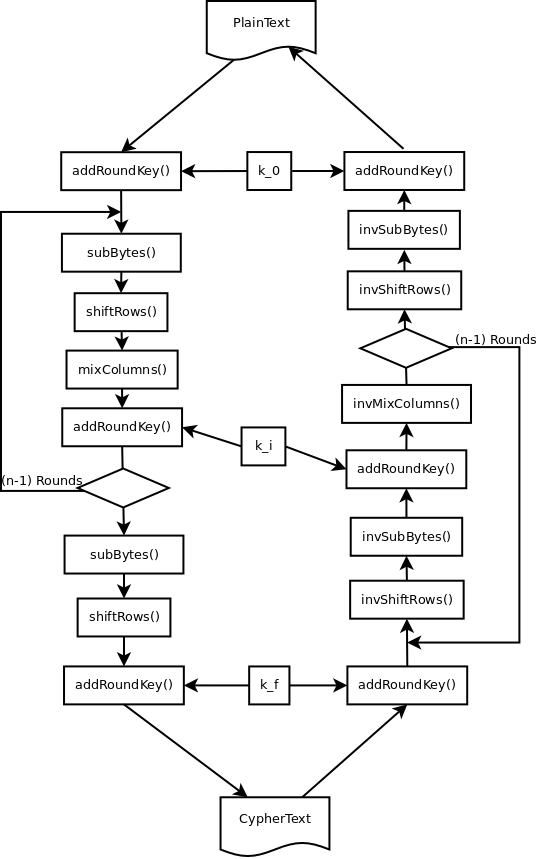
\includegraphics[scale=0.3,keepaspectratio=true]{./images/rijndaelDiagram.png}
 %% Graphic for TeX using PGF
% Title: /home/serguei/src/Papers/Generalized_Rijndael/images/rijndaelDiagram.dia
% Creator: Dia v0.97.2
% CreationDate: Sun Aug 25 21:18:43 2013
% For: serguei
% \usepackage{tikz}
% The following commands are not supported in PSTricks at present
% We define them conditionally, so when they are implemented,
% this pgf file will use them.
\ifx\du\undefined
  \newlength{\du}
\fi
\setlength{\du}{15\unitlength}
\begin{tikzpicture}
\pgftransformxscale{1.000000}
\pgftransformyscale{-1.000000}
\definecolor{dialinecolor}{rgb}{0.000000, 0.000000, 0.000000}
\pgfsetstrokecolor{dialinecolor}
\definecolor{dialinecolor}{rgb}{1.000000, 1.000000, 1.000000}
\pgfsetfillcolor{dialinecolor}
% setfont left to latex
\definecolor{dialinecolor}{rgb}{0.000000, 0.000000, 0.000000}
\pgfsetstrokecolor{dialinecolor}
\node[anchor=west] at (22.350000\du,2.600000\du){Rijdael Schematic};
\definecolor{dialinecolor}{rgb}{1.000000, 1.000000, 1.000000}
\pgfsetfillcolor{dialinecolor}
\fill (15.714800\du,12.969300\du)--(15.714800\du,14.869300\du)--(21.712300\du,14.869300\du)--(21.712300\du,12.969300\du)--cycle;
\pgfsetlinewidth{0.100000\du}
\pgfsetdash{}{0pt}
\pgfsetdash{}{0pt}
\pgfsetmiterjoin
\definecolor{dialinecolor}{rgb}{0.000000, 0.000000, 0.000000}
\pgfsetstrokecolor{dialinecolor}
\draw (15.714800\du,12.969300\du)--(15.714800\du,14.869300\du)--(21.712300\du,14.869300\du)--(21.712300\du,12.969300\du)--cycle;
% setfont left to latex
\definecolor{dialinecolor}{rgb}{0.000000, 0.000000, 0.000000}
\pgfsetstrokecolor{dialinecolor}
\node at (18.713550\du,14.114300\du){addRoundKey()};
\pgfsetlinewidth{0.100000\du}
\pgfsetdash{}{0pt}
\pgfsetdash{}{0pt}
\pgfsetbuttcap
\pgfsetmiterjoin
\pgfsetlinewidth{0.100000\du}
\pgfsetbuttcap
\pgfsetmiterjoin
\pgfsetdash{}{0pt}
\definecolor{dialinecolor}{rgb}{1.000000, 1.000000, 1.000000}
\pgfsetfillcolor{dialinecolor}
\pgfpathmoveto{\pgfpoint{23.000000\du}{5.400000\du}}
\pgfpathlineto{\pgfpoint{28.450000\du}{5.400000\du}}
\pgfpathlineto{\pgfpoint{28.450000\du}{8.014286\du}}
\pgfpathcurveto{\pgfpoint{27.360000\du}{7.578571\du}}{\pgfpoint{26.815000\du}{7.578571\du}}{\pgfpoint{25.725000\du}{8.014286\du}}
\pgfpathcurveto{\pgfpoint{24.635000\du}{8.450000\du}}{\pgfpoint{24.090000\du}{8.450000\du}}{\pgfpoint{23.000000\du}{8.014286\du}}
\pgfpathlineto{\pgfpoint{23.000000\du}{5.400000\du}}
\pgfusepath{fill}
\definecolor{dialinecolor}{rgb}{0.000000, 0.000000, 0.000000}
\pgfsetstrokecolor{dialinecolor}
\pgfpathmoveto{\pgfpoint{23.000000\du}{5.400000\du}}
\pgfpathlineto{\pgfpoint{28.450000\du}{5.400000\du}}
\pgfpathlineto{\pgfpoint{28.450000\du}{8.014286\du}}
\pgfpathcurveto{\pgfpoint{27.360000\du}{7.578571\du}}{\pgfpoint{26.815000\du}{7.578571\du}}{\pgfpoint{25.725000\du}{8.014286\du}}
\pgfpathcurveto{\pgfpoint{24.635000\du}{8.450000\du}}{\pgfpoint{24.090000\du}{8.450000\du}}{\pgfpoint{23.000000\du}{8.014286\du}}
\pgfpathlineto{\pgfpoint{23.000000\du}{5.400000\du}}
\pgfusepath{stroke}
% setfont left to latex
\definecolor{dialinecolor}{rgb}{0.000000, 0.000000, 0.000000}
\pgfsetstrokecolor{dialinecolor}
\node at (25.725000\du,6.689286\du){PlainText};
\pgfsetlinewidth{0.100000\du}
\pgfsetdash{}{0pt}
\pgfsetdash{}{0pt}
\pgfsetbuttcap
{
\definecolor{dialinecolor}{rgb}{0.000000, 0.000000, 0.000000}
\pgfsetfillcolor{dialinecolor}
% was here!!!
\pgfsetarrowsend{stealth}
\definecolor{dialinecolor}{rgb}{0.000000, 0.000000, 0.000000}
\pgfsetstrokecolor{dialinecolor}
\draw (24.362500\du,8.341070\du)--(18.713600\du,12.969300\du);
}
\definecolor{dialinecolor}{rgb}{1.000000, 1.000000, 1.000000}
\pgfsetfillcolor{dialinecolor}
\fill (15.750000\du,17.050000\du)--(15.750000\du,18.950000\du)--(21.700000\du,18.950000\du)--(21.700000\du,17.050000\du)--cycle;
\pgfsetlinewidth{0.100000\du}
\pgfsetdash{}{0pt}
\pgfsetdash{}{0pt}
\pgfsetmiterjoin
\definecolor{dialinecolor}{rgb}{0.000000, 0.000000, 0.000000}
\pgfsetstrokecolor{dialinecolor}
\draw (15.750000\du,17.050000\du)--(15.750000\du,18.950000\du)--(21.700000\du,18.950000\du)--(21.700000\du,17.050000\du)--cycle;
% setfont left to latex
\definecolor{dialinecolor}{rgb}{0.000000, 0.000000, 0.000000}
\pgfsetstrokecolor{dialinecolor}
\node at (18.725000\du,18.195000\du){subBytes()};
\definecolor{dialinecolor}{rgb}{1.000000, 1.000000, 1.000000}
\pgfsetfillcolor{dialinecolor}
\fill (16.386800\du,20.027100\du)--(16.386800\du,21.927100\du)--(21.031800\du,21.927100\du)--(21.031800\du,20.027100\du)--cycle;
\pgfsetlinewidth{0.100000\du}
\pgfsetdash{}{0pt}
\pgfsetdash{}{0pt}
\pgfsetmiterjoin
\definecolor{dialinecolor}{rgb}{0.000000, 0.000000, 0.000000}
\pgfsetstrokecolor{dialinecolor}
\draw (16.386800\du,20.027100\du)--(16.386800\du,21.927100\du)--(21.031800\du,21.927100\du)--(21.031800\du,20.027100\du)--cycle;
% setfont left to latex
\definecolor{dialinecolor}{rgb}{0.000000, 0.000000, 0.000000}
\pgfsetstrokecolor{dialinecolor}
\node at (18.709300\du,21.172100\du){shiftRows()};
\definecolor{dialinecolor}{rgb}{1.000000, 1.000000, 1.000000}
\pgfsetfillcolor{dialinecolor}
\fill (15.980200\du,22.900000\du)--(15.980200\du,24.800000\du)--(21.542700\du,24.800000\du)--(21.542700\du,22.900000\du)--cycle;
\pgfsetlinewidth{0.100000\du}
\pgfsetdash{}{0pt}
\pgfsetdash{}{0pt}
\pgfsetmiterjoin
\definecolor{dialinecolor}{rgb}{0.000000, 0.000000, 0.000000}
\pgfsetstrokecolor{dialinecolor}
\draw (15.980200\du,22.900000\du)--(15.980200\du,24.800000\du)--(21.542700\du,24.800000\du)--(21.542700\du,22.900000\du)--cycle;
% setfont left to latex
\definecolor{dialinecolor}{rgb}{0.000000, 0.000000, 0.000000}
\pgfsetstrokecolor{dialinecolor}
\node at (18.761450\du,24.045000\du){mixColumns()};
\definecolor{dialinecolor}{rgb}{1.000000, 1.000000, 1.000000}
\pgfsetfillcolor{dialinecolor}
\fill (15.766300\du,25.788600\du)--(15.766300\du,27.688600\du)--(21.763800\du,27.688600\du)--(21.763800\du,25.788600\du)--cycle;
\pgfsetlinewidth{0.100000\du}
\pgfsetdash{}{0pt}
\pgfsetdash{}{0pt}
\pgfsetmiterjoin
\definecolor{dialinecolor}{rgb}{0.000000, 0.000000, 0.000000}
\pgfsetstrokecolor{dialinecolor}
\draw (15.766300\du,25.788600\du)--(15.766300\du,27.688600\du)--(21.763800\du,27.688600\du)--(21.763800\du,25.788600\du)--cycle;
% setfont left to latex
\definecolor{dialinecolor}{rgb}{0.000000, 0.000000, 0.000000}
\pgfsetstrokecolor{dialinecolor}
\node at (18.765050\du,26.933600\du){addRoundKey()};
\definecolor{dialinecolor}{rgb}{1.000000, 1.000000, 1.000000}
\pgfsetfillcolor{dialinecolor}
\fill (15.882200\du,32.160000\du)--(15.882200\du,34.060000\du)--(21.832200\du,34.060000\du)--(21.832200\du,32.160000\du)--cycle;
\pgfsetlinewidth{0.100000\du}
\pgfsetdash{}{0pt}
\pgfsetdash{}{0pt}
\pgfsetmiterjoin
\definecolor{dialinecolor}{rgb}{0.000000, 0.000000, 0.000000}
\pgfsetstrokecolor{dialinecolor}
\draw (15.882200\du,32.160000\du)--(15.882200\du,34.060000\du)--(21.832200\du,34.060000\du)--(21.832200\du,32.160000\du)--cycle;
% setfont left to latex
\definecolor{dialinecolor}{rgb}{0.000000, 0.000000, 0.000000}
\pgfsetstrokecolor{dialinecolor}
\node at (18.857200\du,33.305000\du){subBytes()};
\definecolor{dialinecolor}{rgb}{1.000000, 1.000000, 1.000000}
\pgfsetfillcolor{dialinecolor}
\fill (16.535800\du,35.310000\du)--(16.535800\du,37.210000\du)--(21.180800\du,37.210000\du)--(21.180800\du,35.310000\du)--cycle;
\pgfsetlinewidth{0.100000\du}
\pgfsetdash{}{0pt}
\pgfsetdash{}{0pt}
\pgfsetmiterjoin
\definecolor{dialinecolor}{rgb}{0.000000, 0.000000, 0.000000}
\pgfsetstrokecolor{dialinecolor}
\draw (16.535800\du,35.310000\du)--(16.535800\du,37.210000\du)--(21.180800\du,37.210000\du)--(21.180800\du,35.310000\du)--cycle;
% setfont left to latex
\definecolor{dialinecolor}{rgb}{0.000000, 0.000000, 0.000000}
\pgfsetstrokecolor{dialinecolor}
\node at (18.858300\du,36.455000\du){shiftRows()};
\definecolor{dialinecolor}{rgb}{1.000000, 1.000000, 1.000000}
\pgfsetfillcolor{dialinecolor}
\fill (15.855100\du,38.710000\du)--(15.855100\du,40.610000\du)--(21.852600\du,40.610000\du)--(21.852600\du,38.710000\du)--cycle;
\pgfsetlinewidth{0.100000\du}
\pgfsetdash{}{0pt}
\pgfsetdash{}{0pt}
\pgfsetmiterjoin
\definecolor{dialinecolor}{rgb}{0.000000, 0.000000, 0.000000}
\pgfsetstrokecolor{dialinecolor}
\draw (15.855100\du,38.710000\du)--(15.855100\du,40.610000\du)--(21.852600\du,40.610000\du)--(21.852600\du,38.710000\du)--cycle;
% setfont left to latex
\definecolor{dialinecolor}{rgb}{0.000000, 0.000000, 0.000000}
\pgfsetstrokecolor{dialinecolor}
\node at (18.853850\du,39.855000\du){addRoundKey()};
\pgfsetlinewidth{0.100000\du}
\pgfsetdash{}{0pt}
\pgfsetdash{}{0pt}
\pgfsetbuttcap
{
\definecolor{dialinecolor}{rgb}{0.000000, 0.000000, 0.000000}
\pgfsetfillcolor{dialinecolor}
% was here!!!
\pgfsetarrowsend{stealth}
\definecolor{dialinecolor}{rgb}{0.000000, 0.000000, 0.000000}
\pgfsetstrokecolor{dialinecolor}
\draw (18.713600\du,14.869300\du)--(18.725000\du,17.050000\du);
}
\pgfsetlinewidth{0.100000\du}
\pgfsetdash{}{0pt}
\pgfsetdash{}{0pt}
\pgfsetbuttcap
{
\definecolor{dialinecolor}{rgb}{0.000000, 0.000000, 0.000000}
\pgfsetfillcolor{dialinecolor}
% was here!!!
\pgfsetarrowsend{stealth}
\definecolor{dialinecolor}{rgb}{0.000000, 0.000000, 0.000000}
\pgfsetstrokecolor{dialinecolor}
\draw (18.725000\du,18.950000\du)--(18.709300\du,20.027100\du);
}
\pgfsetlinewidth{0.100000\du}
\pgfsetdash{}{0pt}
\pgfsetdash{}{0pt}
\pgfsetbuttcap
{
\definecolor{dialinecolor}{rgb}{0.000000, 0.000000, 0.000000}
\pgfsetfillcolor{dialinecolor}
% was here!!!
\pgfsetarrowsend{stealth}
\definecolor{dialinecolor}{rgb}{0.000000, 0.000000, 0.000000}
\pgfsetstrokecolor{dialinecolor}
\draw (18.736393\du,21.977046\du)--(18.761400\du,22.900000\du);
}
\pgfsetlinewidth{0.100000\du}
\pgfsetdash{}{0pt}
\pgfsetdash{}{0pt}
\pgfsetbuttcap
{
\definecolor{dialinecolor}{rgb}{0.000000, 0.000000, 0.000000}
\pgfsetfillcolor{dialinecolor}
% was here!!!
\pgfsetarrowsend{stealth}
\definecolor{dialinecolor}{rgb}{0.000000, 0.000000, 0.000000}
\pgfsetstrokecolor{dialinecolor}
\draw (18.761400\du,24.800000\du)--(18.765100\du,25.788600\du);
}
\pgfsetlinewidth{0.100000\du}
\pgfsetdash{}{0pt}
\pgfsetdash{}{0pt}
\pgfsetbuttcap
{
\definecolor{dialinecolor}{rgb}{0.000000, 0.000000, 0.000000}
\pgfsetfillcolor{dialinecolor}
% was here!!!
\pgfsetarrowsend{stealth}
\definecolor{dialinecolor}{rgb}{0.000000, 0.000000, 0.000000}
\pgfsetstrokecolor{dialinecolor}
\draw (18.765100\du,27.688600\du)--(18.857200\du,32.160000\du);
}
\pgfsetlinewidth{0.100000\du}
\pgfsetdash{}{0pt}
\pgfsetdash{}{0pt}
\pgfsetbuttcap
{
\definecolor{dialinecolor}{rgb}{0.000000, 0.000000, 0.000000}
\pgfsetfillcolor{dialinecolor}
% was here!!!
\pgfsetarrowsend{stealth}
\definecolor{dialinecolor}{rgb}{0.000000, 0.000000, 0.000000}
\pgfsetstrokecolor{dialinecolor}
\draw (18.857200\du,34.060000\du)--(18.858300\du,35.310000\du);
}
\pgfsetlinewidth{0.100000\du}
\pgfsetdash{}{0pt}
\pgfsetdash{}{0pt}
\pgfsetbuttcap
{
\definecolor{dialinecolor}{rgb}{0.000000, 0.000000, 0.000000}
\pgfsetfillcolor{dialinecolor}
% was here!!!
\pgfsetarrowsend{stealth}
\definecolor{dialinecolor}{rgb}{0.000000, 0.000000, 0.000000}
\pgfsetstrokecolor{dialinecolor}
\draw (18.858300\du,37.210000\du)--(18.853800\du,38.710000\du);
}
\pgfsetlinewidth{0.100000\du}
\pgfsetdash{}{0pt}
\pgfsetdash{}{0pt}
\pgfsetbuttcap
{
\definecolor{dialinecolor}{rgb}{0.000000, 0.000000, 0.000000}
\pgfsetfillcolor{dialinecolor}
% was here!!!
\pgfsetarrowsend{stealth}
\definecolor{dialinecolor}{rgb}{0.000000, 0.000000, 0.000000}
\pgfsetstrokecolor{dialinecolor}
\draw (18.853800\du,40.610000\du)--(25.052500\du,45.260000\du);
}
\definecolor{dialinecolor}{rgb}{1.000000, 1.000000, 1.000000}
\pgfsetfillcolor{dialinecolor}
\fill (25.032000\du,12.961400\du)--(25.032000\du,14.861400\du)--(27.229500\du,14.861400\du)--(27.229500\du,12.961400\du)--cycle;
\pgfsetlinewidth{0.100000\du}
\pgfsetdash{}{0pt}
\pgfsetdash{}{0pt}
\pgfsetmiterjoin
\definecolor{dialinecolor}{rgb}{0.000000, 0.000000, 0.000000}
\pgfsetstrokecolor{dialinecolor}
\draw (25.032000\du,12.961400\du)--(25.032000\du,14.861400\du)--(27.229500\du,14.861400\du)--(27.229500\du,12.961400\du)--cycle;
% setfont left to latex
\definecolor{dialinecolor}{rgb}{0.000000, 0.000000, 0.000000}
\pgfsetstrokecolor{dialinecolor}
\node at (26.130750\du,14.106400\du){k\_0};
\definecolor{dialinecolor}{rgb}{1.000000, 1.000000, 1.000000}
\pgfsetfillcolor{dialinecolor}
\fill (24.741100\du,26.746400\du)--(24.741100\du,28.646400\du)--(26.936100\du,28.646400\du)--(26.936100\du,26.746400\du)--cycle;
\pgfsetlinewidth{0.100000\du}
\pgfsetdash{}{0pt}
\pgfsetdash{}{0pt}
\pgfsetmiterjoin
\definecolor{dialinecolor}{rgb}{0.000000, 0.000000, 0.000000}
\pgfsetstrokecolor{dialinecolor}
\draw (24.741100\du,26.746400\du)--(24.741100\du,28.646400\du)--(26.936100\du,28.646400\du)--(26.936100\du,26.746400\du)--cycle;
% setfont left to latex
\definecolor{dialinecolor}{rgb}{0.000000, 0.000000, 0.000000}
\pgfsetstrokecolor{dialinecolor}
\node at (25.838600\du,27.891400\du){k\_i};
\definecolor{dialinecolor}{rgb}{1.000000, 1.000000, 1.000000}
\pgfsetfillcolor{dialinecolor}
\fill (25.123200\du,38.711400\du)--(25.123200\du,40.611400\du)--(27.138200\du,40.611400\du)--(27.138200\du,38.711400\du)--cycle;
\pgfsetlinewidth{0.100000\du}
\pgfsetdash{}{0pt}
\pgfsetdash{}{0pt}
\pgfsetmiterjoin
\definecolor{dialinecolor}{rgb}{0.000000, 0.000000, 0.000000}
\pgfsetstrokecolor{dialinecolor}
\draw (25.123200\du,38.711400\du)--(25.123200\du,40.611400\du)--(27.138200\du,40.611400\du)--(27.138200\du,38.711400\du)--cycle;
% setfont left to latex
\definecolor{dialinecolor}{rgb}{0.000000, 0.000000, 0.000000}
\pgfsetstrokecolor{dialinecolor}
\node at (26.130700\du,39.856400\du){k\_f};
\pgfsetlinewidth{0.100000\du}
\pgfsetdash{}{0pt}
\pgfsetdash{}{0pt}
\pgfsetbuttcap
{
\definecolor{dialinecolor}{rgb}{0.000000, 0.000000, 0.000000}
\pgfsetfillcolor{dialinecolor}
% was here!!!
\pgfsetarrowsend{stealth}
\definecolor{dialinecolor}{rgb}{0.000000, 0.000000, 0.000000}
\pgfsetstrokecolor{dialinecolor}
\draw (25.032000\du,13.911400\du)--(21.712300\du,13.919300\du);
}
\pgfsetlinewidth{0.100000\du}
\pgfsetdash{}{0pt}
\pgfsetdash{}{0pt}
\pgfsetbuttcap
{
\definecolor{dialinecolor}{rgb}{0.000000, 0.000000, 0.000000}
\pgfsetfillcolor{dialinecolor}
% was here!!!
\pgfsetarrowsend{stealth}
\definecolor{dialinecolor}{rgb}{0.000000, 0.000000, 0.000000}
\pgfsetstrokecolor{dialinecolor}
\draw (24.741100\du,27.696400\du)--(21.763800\du,26.738600\du);
}
\pgfsetlinewidth{0.100000\du}
\pgfsetdash{}{0pt}
\pgfsetdash{}{0pt}
\pgfsetbuttcap
{
\definecolor{dialinecolor}{rgb}{0.000000, 0.000000, 0.000000}
\pgfsetfillcolor{dialinecolor}
% was here!!!
\pgfsetarrowsend{stealth}
\definecolor{dialinecolor}{rgb}{0.000000, 0.000000, 0.000000}
\pgfsetstrokecolor{dialinecolor}
\draw (25.123200\du,39.661400\du)--(21.852600\du,39.660000\du);
}
\pgfsetlinewidth{0.100000\du}
\pgfsetdash{}{0pt}
\pgfsetdash{}{0pt}
\pgfsetmiterjoin
\pgfsetbuttcap
{
\definecolor{dialinecolor}{rgb}{0.000000, 0.000000, 0.000000}
\pgfsetfillcolor{dialinecolor}
% was here!!!
\pgfsetarrowsend{stealth}
{\pgfsetcornersarced{\pgfpoint{0.000000\du}{0.000000\du}}\definecolor{dialinecolor}{rgb}{0.000000, 0.000000, 0.000000}
\pgfsetstrokecolor{dialinecolor}
\draw (18.811100\du,29.924300\du)--(12.700000\du,29.924300\du)--(12.700000\du,15.959600\du)--(18.719300\du,15.959600\du);
}}
% setfont left to latex
\definecolor{dialinecolor}{rgb}{0.000000, 0.000000, 0.000000}
\pgfsetstrokecolor{dialinecolor}
\node[anchor=west] at (12.700000\du,29.600000\du){(n-1) Rounds};
\pgfsetlinewidth{0.100000\du}
\pgfsetdash{}{0pt}
\pgfsetdash{}{0pt}
\pgfsetbuttcap
\pgfsetmiterjoin
\pgfsetlinewidth{0.100000\du}
\pgfsetbuttcap
\pgfsetmiterjoin
\pgfsetdash{}{0pt}
\definecolor{dialinecolor}{rgb}{1.000000, 1.000000, 1.000000}
\pgfsetfillcolor{dialinecolor}
\pgfpathmoveto{\pgfpoint{23.690000\du}{45.260000\du}}
\pgfpathlineto{\pgfpoint{29.140000\du}{45.260000\du}}
\pgfpathlineto{\pgfpoint{29.140000\du}{47.874286\du}}
\pgfpathcurveto{\pgfpoint{28.050000\du}{47.438571\du}}{\pgfpoint{27.505000\du}{47.438571\du}}{\pgfpoint{26.415000\du}{47.874286\du}}
\pgfpathcurveto{\pgfpoint{25.325000\du}{48.310000\du}}{\pgfpoint{24.780000\du}{48.310000\du}}{\pgfpoint{23.690000\du}{47.874286\du}}
\pgfpathlineto{\pgfpoint{23.690000\du}{45.260000\du}}
\pgfusepath{fill}
\definecolor{dialinecolor}{rgb}{0.000000, 0.000000, 0.000000}
\pgfsetstrokecolor{dialinecolor}
\pgfpathmoveto{\pgfpoint{23.690000\du}{45.260000\du}}
\pgfpathlineto{\pgfpoint{29.140000\du}{45.260000\du}}
\pgfpathlineto{\pgfpoint{29.140000\du}{47.874286\du}}
\pgfpathcurveto{\pgfpoint{28.050000\du}{47.438571\du}}{\pgfpoint{27.505000\du}{47.438571\du}}{\pgfpoint{26.415000\du}{47.874286\du}}
\pgfpathcurveto{\pgfpoint{25.325000\du}{48.310000\du}}{\pgfpoint{24.780000\du}{48.310000\du}}{\pgfpoint{23.690000\du}{47.874286\du}}
\pgfpathlineto{\pgfpoint{23.690000\du}{45.260000\du}}
\pgfusepath{stroke}
% setfont left to latex
\definecolor{dialinecolor}{rgb}{0.000000, 0.000000, 0.000000}
\pgfsetstrokecolor{dialinecolor}
\node at (26.415000\du,46.549286\du){CypherText};
\definecolor{dialinecolor}{rgb}{1.000000, 1.000000, 1.000000}
\pgfsetfillcolor{dialinecolor}
\fill (30.040000\du,38.710000\du)--(30.040000\du,40.610000\du)--(36.037500\du,40.610000\du)--(36.037500\du,38.710000\du)--cycle;
\pgfsetlinewidth{0.100000\du}
\pgfsetdash{}{0pt}
\pgfsetdash{}{0pt}
\pgfsetmiterjoin
\definecolor{dialinecolor}{rgb}{0.000000, 0.000000, 0.000000}
\pgfsetstrokecolor{dialinecolor}
\draw (30.040000\du,38.710000\du)--(30.040000\du,40.610000\du)--(36.037500\du,40.610000\du)--(36.037500\du,38.710000\du)--cycle;
% setfont left to latex
\definecolor{dialinecolor}{rgb}{0.000000, 0.000000, 0.000000}
\pgfsetstrokecolor{dialinecolor}
\node at (33.038750\du,39.855000\du){addRoundKey()};
\pgfsetlinewidth{0.100000\du}
\pgfsetdash{}{0pt}
\pgfsetdash{}{0pt}
\pgfsetbuttcap
{
\definecolor{dialinecolor}{rgb}{0.000000, 0.000000, 0.000000}
\pgfsetfillcolor{dialinecolor}
% was here!!!
\pgfsetarrowsend{stealth}
\definecolor{dialinecolor}{rgb}{0.000000, 0.000000, 0.000000}
\pgfsetstrokecolor{dialinecolor}
\draw (33.038700\du,38.710000\du)--(33.019200\du,36.319300\du);
}
\pgfsetlinewidth{0.100000\du}
\pgfsetdash{}{0pt}
\pgfsetdash{}{0pt}
\pgfsetbuttcap
{
\definecolor{dialinecolor}{rgb}{0.000000, 0.000000, 0.000000}
\pgfsetfillcolor{dialinecolor}
% was here!!!
\pgfsetarrowsend{stealth}
\definecolor{dialinecolor}{rgb}{0.000000, 0.000000, 0.000000}
\pgfsetstrokecolor{dialinecolor}
\draw (27.138200\du,39.661400\du)--(30.040000\du,39.660000\du);
}
\definecolor{dialinecolor}{rgb}{1.000000, 1.000000, 1.000000}
\pgfsetfillcolor{dialinecolor}
\fill (30.206400\du,31.269300\du)--(30.206400\du,33.169300\du)--(35.786400\du,33.169300\du)--(35.786400\du,31.269300\du)--cycle;
\pgfsetlinewidth{0.100000\du}
\pgfsetdash{}{0pt}
\pgfsetdash{}{0pt}
\pgfsetmiterjoin
\definecolor{dialinecolor}{rgb}{0.000000, 0.000000, 0.000000}
\pgfsetstrokecolor{dialinecolor}
\draw (30.206400\du,31.269300\du)--(30.206400\du,33.169300\du)--(35.786400\du,33.169300\du)--(35.786400\du,31.269300\du)--cycle;
% setfont left to latex
\definecolor{dialinecolor}{rgb}{0.000000, 0.000000, 0.000000}
\pgfsetstrokecolor{dialinecolor}
\node at (32.996400\du,32.414300\du){invSubBytes()};
\pgfsetlinewidth{0.100000\du}
\pgfsetdash{}{0pt}
\pgfsetdash{}{0pt}
\pgfsetbuttcap
{
\definecolor{dialinecolor}{rgb}{0.000000, 0.000000, 0.000000}
\pgfsetfillcolor{dialinecolor}
% was here!!!
\pgfsetarrowsend{stealth}
\definecolor{dialinecolor}{rgb}{0.000000, 0.000000, 0.000000}
\pgfsetstrokecolor{dialinecolor}
\draw (33.019200\du,34.419300\du)--(32.996400\du,33.169300\du);
}
\definecolor{dialinecolor}{rgb}{1.000000, 1.000000, 1.000000}
\pgfsetfillcolor{dialinecolor}
\fill (29.994200\du,27.890700\du)--(29.994200\du,29.790700\du)--(35.991700\du,29.790700\du)--(35.991700\du,27.890700\du)--cycle;
\pgfsetlinewidth{0.100000\du}
\pgfsetdash{}{0pt}
\pgfsetdash{}{0pt}
\pgfsetmiterjoin
\definecolor{dialinecolor}{rgb}{0.000000, 0.000000, 0.000000}
\pgfsetstrokecolor{dialinecolor}
\draw (29.994200\du,27.890700\du)--(29.994200\du,29.790700\du)--(35.991700\du,29.790700\du)--(35.991700\du,27.890700\du)--cycle;
% setfont left to latex
\definecolor{dialinecolor}{rgb}{0.000000, 0.000000, 0.000000}
\pgfsetstrokecolor{dialinecolor}
\node at (32.992950\du,29.035700\du){addRoundKey()};
\pgfsetlinewidth{0.100000\du}
\pgfsetdash{}{0pt}
\pgfsetdash{}{0pt}
\pgfsetbuttcap
{
\definecolor{dialinecolor}{rgb}{0.000000, 0.000000, 0.000000}
\pgfsetfillcolor{dialinecolor}
% was here!!!
\pgfsetarrowsend{stealth}
\definecolor{dialinecolor}{rgb}{0.000000, 0.000000, 0.000000}
\pgfsetstrokecolor{dialinecolor}
\draw (32.996400\du,31.269300\du)--(32.992900\du,29.790700\du);
}
\definecolor{dialinecolor}{rgb}{1.000000, 1.000000, 1.000000}
\pgfsetfillcolor{dialinecolor}
\fill (29.773100\du,24.619300\du)--(29.773100\du,26.519300\du)--(36.228100\du,26.519300\du)--(36.228100\du,24.619300\du)--cycle;
\pgfsetlinewidth{0.100000\du}
\pgfsetdash{}{0pt}
\pgfsetdash{}{0pt}
\pgfsetmiterjoin
\definecolor{dialinecolor}{rgb}{0.000000, 0.000000, 0.000000}
\pgfsetstrokecolor{dialinecolor}
\draw (29.773100\du,24.619300\du)--(29.773100\du,26.519300\du)--(36.228100\du,26.519300\du)--(36.228100\du,24.619300\du)--cycle;
% setfont left to latex
\definecolor{dialinecolor}{rgb}{0.000000, 0.000000, 0.000000}
\pgfsetstrokecolor{dialinecolor}
\node at (33.000600\du,25.764300\du){invMixColumns()};
\pgfsetlinewidth{0.100000\du}
\pgfsetdash{}{0pt}
\pgfsetdash{}{0pt}
\pgfsetbuttcap
{
\definecolor{dialinecolor}{rgb}{0.000000, 0.000000, 0.000000}
\pgfsetfillcolor{dialinecolor}
% was here!!!
\pgfsetarrowsend{stealth}
\definecolor{dialinecolor}{rgb}{0.000000, 0.000000, 0.000000}
\pgfsetstrokecolor{dialinecolor}
\draw (32.992900\du,27.890700\du)--(33.000600\du,26.519300\du);
}
\pgfsetlinewidth{0.100000\du}
\pgfsetdash{}{0pt}
\pgfsetdash{}{0pt}
\pgfsetmiterjoin
\pgfsetbuttcap
{
\definecolor{dialinecolor}{rgb}{0.000000, 0.000000, 0.000000}
\pgfsetfillcolor{dialinecolor}
% was here!!!
\pgfsetarrowsend{stealth}
{\pgfsetcornersarced{\pgfpoint{0.000000\du}{0.000000\du}}\definecolor{dialinecolor}{rgb}{0.000000, 0.000000, 0.000000}
\pgfsetstrokecolor{dialinecolor}
\draw (32.949000\du,22.725800\du)--(38.650000\du,22.725800\du)--(38.650000\du,37.514600\du)--(33.029000\du,37.514600\du);
}}
% setfont left to latex
\definecolor{dialinecolor}{rgb}{0.000000, 0.000000, 0.000000}
\pgfsetstrokecolor{dialinecolor}
\node[anchor=west] at (35.450000\du,22.550000\du){(n-1) Rounds};
\definecolor{dialinecolor}{rgb}{1.000000, 1.000000, 1.000000}
\pgfsetfillcolor{dialinecolor}
\fill (30.178000\du,34.419300\du)--(30.178000\du,36.319300\du)--(35.860500\du,36.319300\du)--(35.860500\du,34.419300\du)--cycle;
\pgfsetlinewidth{0.100000\du}
\pgfsetdash{}{0pt}
\pgfsetdash{}{0pt}
\pgfsetmiterjoin
\definecolor{dialinecolor}{rgb}{0.000000, 0.000000, 0.000000}
\pgfsetstrokecolor{dialinecolor}
\draw (30.178000\du,34.419300\du)--(30.178000\du,36.319300\du)--(35.860500\du,36.319300\du)--(35.860500\du,34.419300\du)--cycle;
% setfont left to latex
\definecolor{dialinecolor}{rgb}{0.000000, 0.000000, 0.000000}
\pgfsetstrokecolor{dialinecolor}
\node at (33.019250\du,35.564300\du){invShiftRows()};
\definecolor{dialinecolor}{rgb}{1.000000, 1.000000, 1.000000}
\pgfsetfillcolor{dialinecolor}
\fill (30.056300\du,18.932300\du)--(30.056300\du,20.832300\du)--(35.738800\du,20.832300\du)--(35.738800\du,18.932300\du)--cycle;
\pgfsetlinewidth{0.100000\du}
\pgfsetdash{}{0pt}
\pgfsetdash{}{0pt}
\pgfsetmiterjoin
\definecolor{dialinecolor}{rgb}{0.000000, 0.000000, 0.000000}
\pgfsetstrokecolor{dialinecolor}
\draw (30.056300\du,18.932300\du)--(30.056300\du,20.832300\du)--(35.738800\du,20.832300\du)--(35.738800\du,18.932300\du)--cycle;
% setfont left to latex
\definecolor{dialinecolor}{rgb}{0.000000, 0.000000, 0.000000}
\pgfsetstrokecolor{dialinecolor}
\node at (32.897550\du,20.077300\du){invShiftRows()};
\pgfsetlinewidth{0.100000\du}
\pgfsetdash{}{0pt}
\pgfsetdash{}{0pt}
\pgfsetbuttcap
{
\definecolor{dialinecolor}{rgb}{0.000000, 0.000000, 0.000000}
\pgfsetfillcolor{dialinecolor}
% was here!!!
\pgfsetarrowsend{stealth}
\definecolor{dialinecolor}{rgb}{0.000000, 0.000000, 0.000000}
\pgfsetstrokecolor{dialinecolor}
\draw (33.000600\du,24.619300\du)--(32.897500\du,20.832300\du);
}
\definecolor{dialinecolor}{rgb}{1.000000, 1.000000, 1.000000}
\pgfsetfillcolor{dialinecolor}
\fill (30.091200\du,15.905800\du)--(30.091200\du,17.805800\du)--(35.671200\du,17.805800\du)--(35.671200\du,15.905800\du)--cycle;
\pgfsetlinewidth{0.100000\du}
\pgfsetdash{}{0pt}
\pgfsetdash{}{0pt}
\pgfsetmiterjoin
\definecolor{dialinecolor}{rgb}{0.000000, 0.000000, 0.000000}
\pgfsetstrokecolor{dialinecolor}
\draw (30.091200\du,15.905800\du)--(30.091200\du,17.805800\du)--(35.671200\du,17.805800\du)--(35.671200\du,15.905800\du)--cycle;
% setfont left to latex
\definecolor{dialinecolor}{rgb}{0.000000, 0.000000, 0.000000}
\pgfsetstrokecolor{dialinecolor}
\node at (32.881200\du,17.050800\du){invSubBytes()};
\definecolor{dialinecolor}{rgb}{1.000000, 1.000000, 1.000000}
\pgfsetfillcolor{dialinecolor}
\fill (29.890600\du,12.960000\du)--(29.890600\du,14.860000\du)--(35.888100\du,14.860000\du)--(35.888100\du,12.960000\du)--cycle;
\pgfsetlinewidth{0.100000\du}
\pgfsetdash{}{0pt}
\pgfsetdash{}{0pt}
\pgfsetmiterjoin
\definecolor{dialinecolor}{rgb}{0.000000, 0.000000, 0.000000}
\pgfsetstrokecolor{dialinecolor}
\draw (29.890600\du,12.960000\du)--(29.890600\du,14.860000\du)--(35.888100\du,14.860000\du)--(35.888100\du,12.960000\du)--cycle;
% setfont left to latex
\definecolor{dialinecolor}{rgb}{0.000000, 0.000000, 0.000000}
\pgfsetstrokecolor{dialinecolor}
\node at (32.889350\du,14.105000\du){addRoundKey()};
\pgfsetlinewidth{0.100000\du}
\pgfsetdash{}{0pt}
\pgfsetdash{}{0pt}
\pgfsetbuttcap
{
\definecolor{dialinecolor}{rgb}{0.000000, 0.000000, 0.000000}
\pgfsetfillcolor{dialinecolor}
% was here!!!
\pgfsetarrowsend{stealth}
\definecolor{dialinecolor}{rgb}{0.000000, 0.000000, 0.000000}
\pgfsetstrokecolor{dialinecolor}
\draw (32.897500\du,18.932300\du)--(32.889052\du,17.856028\du);
}
\pgfsetlinewidth{0.100000\du}
\pgfsetdash{}{0pt}
\pgfsetdash{}{0pt}
\pgfsetbuttcap
{
\definecolor{dialinecolor}{rgb}{0.000000, 0.000000, 0.000000}
\pgfsetfillcolor{dialinecolor}
% was here!!!
\pgfsetarrowsend{stealth}
\definecolor{dialinecolor}{rgb}{0.000000, 0.000000, 0.000000}
\pgfsetstrokecolor{dialinecolor}
\draw (32.885310\du,15.855464\du)--(32.889400\du,14.860000\du);
}
\pgfsetlinewidth{0.100000\du}
\pgfsetdash{}{0pt}
\pgfsetdash{}{0pt}
\pgfsetbuttcap
{
\definecolor{dialinecolor}{rgb}{0.000000, 0.000000, 0.000000}
\pgfsetfillcolor{dialinecolor}
% was here!!!
\pgfsetarrowsend{stealth}
\definecolor{dialinecolor}{rgb}{0.000000, 0.000000, 0.000000}
\pgfsetstrokecolor{dialinecolor}
\draw (27.278165\du,13.910973\du)--(29.890600\du,13.910000\du);
}
\pgfsetlinewidth{0.100000\du}
\pgfsetdash{}{0pt}
\pgfsetdash{}{0pt}
\pgfsetbuttcap
{
\definecolor{dialinecolor}{rgb}{0.000000, 0.000000, 0.000000}
\pgfsetfillcolor{dialinecolor}
% was here!!!
\pgfsetarrowsend{stealth}
\definecolor{dialinecolor}{rgb}{0.000000, 0.000000, 0.000000}
\pgfsetstrokecolor{dialinecolor}
\draw (26.936100\du,27.696400\du)--(29.994200\du,28.840700\du);
}
\pgfsetlinewidth{0.100000\du}
\pgfsetdash{}{0pt}
\pgfsetdash{}{0pt}
\pgfsetbuttcap
{
\definecolor{dialinecolor}{rgb}{0.000000, 0.000000, 0.000000}
\pgfsetfillcolor{dialinecolor}
% was here!!!
\pgfsetarrowsend{stealth}
\definecolor{dialinecolor}{rgb}{0.000000, 0.000000, 0.000000}
\pgfsetstrokecolor{dialinecolor}
\draw (32.850000\du,12.800000\du)--(27.087500\du,7.687500\du);
}
\pgfsetlinewidth{0.100000\du}
\pgfsetdash{}{0pt}
\pgfsetdash{}{0pt}
\pgfsetbuttcap
{
\definecolor{dialinecolor}{rgb}{0.000000, 0.000000, 0.000000}
\pgfsetfillcolor{dialinecolor}
% was here!!!
\pgfsetarrowsend{stealth}
\definecolor{dialinecolor}{rgb}{0.000000, 0.000000, 0.000000}
\pgfsetstrokecolor{dialinecolor}
\draw (27.777500\du,45.260000\du)--(33.038700\du,40.610000\du);
}
% setfont left to latex
\definecolor{dialinecolor}{rgb}{0.000000, 0.000000, 0.000000}
\pgfsetstrokecolor{dialinecolor}
\node[anchor=west] at (26.150000\du,2.400000\du){};
\definecolor{dialinecolor}{rgb}{1.000000, 1.000000, 1.000000}
\pgfsetfillcolor{dialinecolor}
\fill (18.816879\du,28.801700\du)--(21.101558\du,29.777638\du)--(18.816879\du,30.753576\du)--(16.532200\du,29.777638\du)--cycle;
\pgfsetlinewidth{0.100000\du}
\pgfsetdash{}{0pt}
\pgfsetdash{}{0pt}
\pgfsetmiterjoin
\definecolor{dialinecolor}{rgb}{0.000000, 0.000000, 0.000000}
\pgfsetstrokecolor{dialinecolor}
\draw (18.816879\du,28.801700\du)--(21.101558\du,29.777638\du)--(18.816879\du,30.753576\du)--(16.532200\du,29.777638\du)--cycle;
% setfont left to latex
\definecolor{dialinecolor}{rgb}{0.000000, 0.000000, 0.000000}
\pgfsetstrokecolor{dialinecolor}
\node at (18.816879\du,29.972638\du){};
\definecolor{dialinecolor}{rgb}{1.000000, 1.000000, 1.000000}
\pgfsetfillcolor{dialinecolor}
\fill (32.974679\du,21.810000\du)--(35.259358\du,22.785938\du)--(32.974679\du,23.761876\du)--(30.690000\du,22.785938\du)--cycle;
\pgfsetlinewidth{0.100000\du}
\pgfsetdash{}{0pt}
\pgfsetdash{}{0pt}
\pgfsetmiterjoin
\definecolor{dialinecolor}{rgb}{0.000000, 0.000000, 0.000000}
\pgfsetstrokecolor{dialinecolor}
\draw (32.974679\du,21.810000\du)--(35.259358\du,22.785938\du)--(32.974679\du,23.761876\du)--(30.690000\du,22.785938\du)--cycle;
% setfont left to latex
\definecolor{dialinecolor}{rgb}{0.000000, 0.000000, 0.000000}
\pgfsetstrokecolor{dialinecolor}
\node at (32.974679\du,22.980938\du){};
\end{tikzpicture}

 % rijndaelDiagram.png: 521x887 pixel, 72dpi, 18.38x31.29 cm, bb=0 0 521 887
 \caption{rijndael diagram}
 \label{fig:RijndaelDiagram}
\end{figure}

%%%%%%%%%%%%%%%%%%%%%%%%%%%%%%%%%%%%%%%%%%%%%%%%%%%%%%%%%%%%%%%%%%%%%%%%%%%%%%%
\section{Generalising the schema}\label{sec:generalising}

%%%%%%%%%%%%%%%%%%%%%%%%%%%%%%%%%%%%%%%%%%%%%%%%%%%%%%%%%%%%%%%%%%%%%%%%%%%%%%%
\subsection{key expansion}\label{sec:keyExpansion}
% define s Pseudo-Random Generator (PRG), What a Pseudo-Random Generator is?
The first important operation in the \emph{Rijndael} schema is the \emph{key expansion}. This operation takes the key as a seed to expand it until generate all the subkeys used on each round. In the smaller case of \emph{AES} standard, the 128 bits become expanded to 1280 extra bits to be used like if the key was this size. But why the usage 128 bits in the key, can be trusted like having an independent key 10 times longer? This important mathematical item where this security rest is what is called \emph{Pseudo-Random Generator}, PRG, generating a unique, and always the same, stream of bits from a much shorter seed. Lets define what PRG means:

\begin{definition}\label{def:PRG}
 A \emph{Pseudo-Random Generator} is a function that takes a seed and generates a much larger stream:
 \begin{center}
  \begin{tabular}{llllr}
   PRG: & $\{0,1\}^{s}$ & $\rightarrow$ & $\{0,1\}^n$ & ,where $n \ggg s$\\
  \end{tabular}
 \end{center}
 
\end{definition}
The goal is that the \emph{PRG} must be efficiently computable by a deterministic algorithm and the output of it must look random and unpredictable. In fact, this is the most important property of a \emph{PRG}, the unpredictability. But what predictability means:

\begin{definition}\label{def:unpredictability}
 Given a \emph{PRG} $G: k \rightarrow \{0,1\}^n$ is \emph{predictable} if exist an efficient algorithm \emph{A} such that:
 \begin{equation}
  \underset{k\leftarrow\mathcal{K}}{Pr}\left[A(G(k)|_{1,...,i}) = G(k)|_{i+1}\right]>\frac{1}{2}
+\epsilon \end{equation}
 for a non negligible $\epsilon$
\end{definition}

As an example, a non negligible $\epsilon$ usually is mention as a value $\geqslant\frac{1}{2^{30}}$.

The definition \ref{def:unpredictability} says that for any efficient algorithm, given to this algorithm the $i$ first bits, the probability that this algorithm predicts the next element of the stream is negligible.

The unpredictability of a \emph{PRG} is what gives to it the quality to be \emph{undistinguishable} from a \emph{pure random generator}. Even when the seed space $\mathcal{K}$ of the PRG is much smaller than the space of the output $\{0,1\}^n$.

Like in the PRP, consider an scenario where the adversary has access to a random oracle where the output of this oracle can be the output of the PRG or a truly random stream. The advantage of the adversary to distinguish from where it comes any output it has take can be described as:
\begin{equation}\label{eq:prgAdv}
 {Adv}_{prg}[A,G] = \left|
                     \underset{k\overset{R}{\leftarrow}\mathcal{K}}{Pr}\left[A(G(k))=1\right]-
                     \underset{r\overset{R}{\leftarrow}\{0,1\}^n}{Pr}\left[A(r)=1\right]
                    \right|\in [0,1]
\end{equation}
That means if the probability gets close to 1, the adversary can distinguish $G$ from random; and if it is close to 0 cannot.

\begin{definition}\label{def:advantage}
 Given $G: k \rightarrow \{0,1\}^n$, is a \emph{secure PRG} iff $\forall$ ``efficient statistical test'' the advantage ${Adv}_{prg}[A,G]$ is negligible.
\end{definition}

\todo{We shall proof this definition \ref{def:advantage}}

Following definition \ref{def:unpredictability} about the unpredictability, the $\epsilon$ is $\leqslant\frac{1}{2^{80}}$ to be considered as negligible.

%What can be made with the KeyExpansion() ``playing'' with the parameters (\#rows, \#columns, wordsize) from the key point of view (message things later).
\begin{algorithm}
 \caption{KeyExpansion}
 \label{alg:keyExpansion}
 \begin{algorithmic}[1]
  \REQUIRE nRounds, nRowns, nColumns, wSize, array of words $k_{in}[nRows*nColumns]$
  \ENSURE array of columns(array of words) $k_{out}[nColumns*(nRouns+1)]$
  \STATE i := 0
  \WHILE{$i<nColumns$}
    \STATE $k_{out}[i]$ := column($k_{in}[nRows*(i+c)$ for $c$ in $range(nColumns)]$)
  \ENDWHILE
  \STATE i := nColumns
  \WHILE{$i<nRouns*(nRows+1)$}
    \STATE temp := $k_{out}[i-1]$
    \IF{i mod nColumns == 0}
      \STATE temp := SubWord(RotWord(temp)) $\oplus$ Rcon[i/nColumns]
    \ELSE
      \STATE temp := SubWord(temp)
    \ENDIF
    \STATE $k_{out}[i]$ := $k_{out}[i-nColumns]$ $\oplus$ temp
    \STATE i++
  \ENDWHILE
 \end{algorithmic}
\end{algorithm}

Back to the \emph{key expansion} of the \emph{Rijndael}, and assuming that it is a \emph{secure PRG}, it is time to take a look on the algorithm itself to ``read'' what can be generalized because this is the purpose of this paper. The input of the algorithm \ref{alg:keyExpansion}\footnote{This algorithm has been taken from the version 2 of the AES proposal \cite{Daemen01aes-ammended} that is the same than becomes the NIST standard \cite{AES-FIPS}. Different but equivalent than the algorithm give in the book from the Rijndael authors \cite{Daemen:2002:DR:560131}, published later than the standard} takes, further than the seed key, the number of \emph{rounds}, the number of \emph{rows} and \emph{columns}, and also the \emph{word size}.
%TODO: check how it was the keyExpansion in the first proposal \cite{Daemen98aesproposal:}

All those parameters are necessary to have in the output an expanded key large enough to use all the necessary subparts under each round, as it is shown in the figure \ref{fig:RijndaelDiagram}.

% draw the algorithm as a diagram
\begin{figure}[h!]
\begin{center}
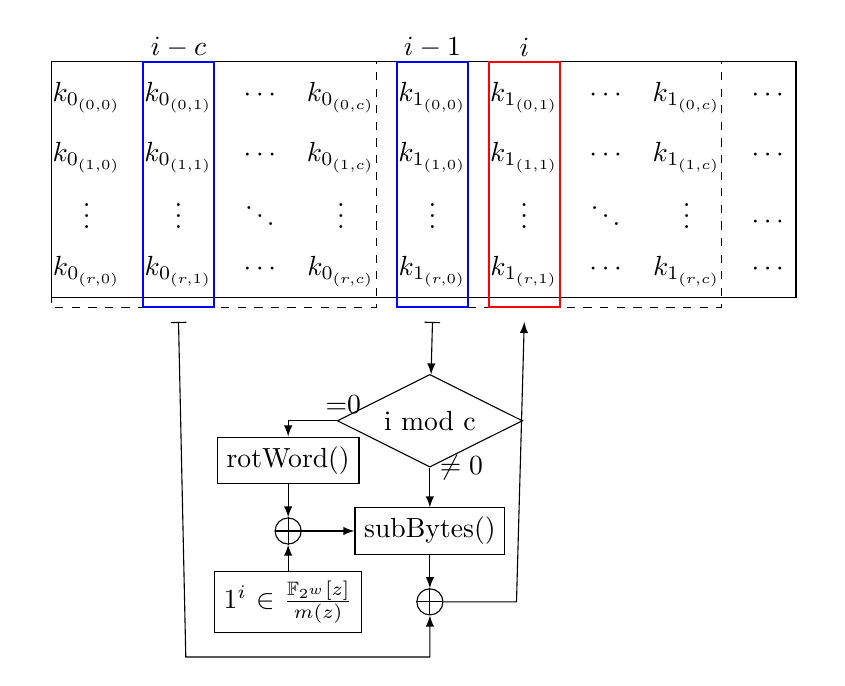
\begin{tikzpicture}[>=latex]
\matrix (k) [matrix of math nodes,nodes = {node style ge},%
              %left delimiter  = (,right delimiter = ),
              column sep=-0.1cm,row sep=-0.5cm,
             ] at (0,0)
        {
          k_{0_{(0,0)}} & k_{0_{(0,1)}} & \cdots & k_{0_{(0,c)}} &
          k_{1_{(0,0)}} & k_{1_{(0,1)}} & \cdots & k_{1_{(0,c)}} &
          \cdots \\%&
          %k_{n_{(0,0)}} & k_{n_{(0,1)}} & \cdots & k_{n_{(0,c)}} \\
          k_{0_{(1,0)}} & k_{0_{(1,1)}} & \cdots & k_{0_{(1,c)}} &
          k_{1_{(1,0)}} & k_{1_{(1,1)}} & \cdots & k_{1_{(1,c)}} &
          \cdots \\%&
          %k_{n_{(1,0)}} & k_{n_{(1,1)}} & \cdots & k_{n_{(1,c)}} \\
          \vdots        & \vdots        & \ddots & \vdots        &
          \vdots        & \vdots        & \ddots & \vdots        &
          \cdots        \\%&
          %\vdots        & \vdots        & \ddots & \vdots        \\
          k_{0_{(r,0)}} & k_{0_{(r,1)}} & \cdots & k_{0_{(r,c)}} &
          k_{1_{(r,0)}} & k_{1_{(r,1)}} & \cdots & k_{1_{(r,c)}} &
          \cdots \\%&
          %k_{n_{(r,0)}} & k_{n_{(r,1)}} & \cdots & k_{n_{(r,c)}}\\
        };
\draw [] (k-1-1.north west) rectangle (k-4-9.south east);
\draw [dashed] (k-1-1.north west) rectangle (k-4-4.south east);
\draw [dashed] (k-1-5.north west) rectangle (k-4-8.south east);
%\draw [dashed] (k-1-10.north west) rectangle (k-4-13.south east);

%boxes to get the necessary columns
\draw [blue,thick] (k-1-2.north west) rectangle (k-4-2.south east);
\draw [blue,thick] (k-1-5.north west) rectangle (k-4-5.south east);
\draw [red,thick] (k-1-6.north west) rectangle (k-4-6.south east);
% 
\node [diamond,draw,aspect=2] (imodc) at (.1,-3) {i mod c};
\node [rectangle,draw] (rotWord) at (-1.7,-3.5) {rotWord()};
\node [circle,draw] (xor1) at (-1.7,-4.4) {};
 \draw [-] (xor1.north) -- (xor1.south);
 \draw [-] (xor1.west) -- (xor1.east);
\node [rectangle,draw] (subBytes) at (.1,-4.4) {subBytes()};
\node [circle,draw] (xor2) at (.1,-5.3) {};
 \draw [-] (xor2.north) -- (xor2.south);
 \draw [-] (xor2.west) -- (xor2.east);
\node [rectangle,draw] (rcon) at (-1.7,-5.3) {$1^i$ $\in$ \Fpnm{w}{z}};%{Rcon[i]};
\node [] (eq0) at (-1,-2.8) {=0};
\node [] (neq) at (.5,-3.6) {$\neq0$};
\node [] (neq) at (k-1-2.north) {$i-c$};
\node [] (neq) at (k-1-5.north) {$i-1$};
\node [] (neq) at (k-1-6.north) {$i$};
% 
% %arrows to set into the algorithm
\draw [|->] (k-4-2.south) -- (-3,-6) -- (.1,-6) -- (xor2.south);
%\draw [|->] (k-4-5.south) -- (-.94,-2) -- (-1.5,-2) -- (imodc);
\draw [|->] (k-4-5.south) -- (imodc);
\draw [->] (imodc.west) -- (-1.7,-3) -- (rotWord.north);
\draw [->] (rotWord.south) -- (xor1.north);
\draw [->] (xor1.east) -- (subBytes.west);
\draw [->] (imodc.south) -- (subBytes.north);
\draw [->] (subBytes.south) -- (xor2.north);
\draw [->] (xor2.east) -- (1.2,-5.3) -- (k-4-6.south);
\draw [->] (rcon.north)--(xor1.south);

\end{tikzpicture}
\caption{Block diagram of the iterative construction of the \emph{Rijndael Key Expansion} as a \emph{PseudoRandomGenerator}, PRG}
\label{fig:keyExpansionDiagram}
\end{center}
\end{figure}

Perhaps a better way to see the algorithm \ref{alg:keyExpansion} is the figure \ref{fig:keyExpansionDiagram}. From steps 1 to 5 in the algorithm it simply ``moves'' the input key to the first part of the generated output. The main part of the algorithm, starts on the step 6 where each column further than the original columns of the key are generated.

With this figure seems to be easier to recognise this iterative algorithm, that is generating the new column $i$ by taking the previous (with may be some transformations when the key size is bigger than the block size) and the one in the same relative position of the previous \emph{subkey}, to do over it some transformations to introduce diffusion and confusion in the newer bits generation.

Each step finish with 3 \emph{xor} operations to catch together all the partials on this step generation. The \emph{xor} operation is the most important operation and is the most used in the lower level of the \emph{Rijndael}. This is one of the bests characteristics of this algorithm.

\begin{itemize}
 \item \todo{subBytes()} is used here (then the SBox) but will be explained deeper in section \ref{sec:subBytes}.
 \item \todo{rotWord()} should be explained here because is not used before and cannot be postponed because is not used later.
 \item \todo{What means to have different number of columns in the message than in the key matrix representation.}
 \item \todo{Explain what is the proposal of the Rcon matrix (or as a recursive function).}
\end{itemize}

% weakness in the key expansion of rijndael when key size != block size
An attack to the \emph{PRG} of the Rijndael is described in \cite{fullaes-192-256} and affects the cases where the size of the key is not the same than the size of the block. Even that, this attack requires up to $2^{99}$ pairs $(m,c)$ and $4$ \emph{related keys}\footnote{\emph{Related keys} means that the \emph{Hamming} distances (definition \ref{def:hammingDistance}) are very short and the difference between one key to another are a few bits that are flipped.}. The recover time of this attack is around $2^{99}$ that is still far away from a weakness to be worried to untrust the algorithm. Also avoiding to use related keys, this attack would not apply.
%FIXME:it may would be developed or rewritten better
%FIXME: check better this article \cite{fullaes-192-256} to review if it have relation with use the number of columns of the block size instead of the key size.

%%%%%%%%%%%%%%%%%%%%%%%%%%%%%%%%%%%%%%%%%%%%%%%%%%%%%%%%%%%%%%%%%%%%%%%%%%%%%%%
\subsection{Rounds}\label{sec:rounds}
% why n rounds and not more, not less?

In the AES proposal of the Rijndael \cite{Daemen01aes-ammended} (section 4.1) the number of rounds is described as a function of the block and the key length, followed by the table:
\begin{equation}\label{tab:nrounds}
%\begin{center}
\begin{tabular}{|c||c|c|c|}
\hline
$N_r$     & $N_b = 4$ & $N_b = 6$ & $N_b = 8$ \\ \hline\hline
$N_k = 4$ &    $10$   &    $12$   &    $14$   \\ \hline
$N_k = 6$ &    $12$   &    $12$   &    $14$   \\ \hline
$N_k = 8$ &    $14$   &    $14$   &    $14$   \\ \hline
\end{tabular}
%\end{center}
\end{equation}

 But is in section 7.6 where is said that this number has been determined by looking in to the most efficient attacks (known at that time) and adding a security margin. That is improved with in section 12.1, where the number of rounds is described by a function:
\begin{equation}\label{eq:nrounds}
 N_r = max(N_k,N_b)+6
\end{equation}
This function means that the number of rounds is the biggest number of columns between the block and the key, plus the security margin set as $6$.

\begin{itemize}
 \item \todo{ But, with this, there isn't a proof of why those sizes yet.}
\end{itemize}



%%%%%%%%%%%%%%%%%%%%%%%%%%%%%%%%%%%%%%%%%%%%%%%%%%%%%%%%%%%%%%%%%%%%%%%%%%%%%%%
\subsection{subBytes}\label{sec:subBytes}

Looking on the schema of the figure \ref{fig:RijndaelDiagram}, skipping the \emph{addRoundKey} with $k_0$ --that will be explain later in section \ref{sec:addRoundKey}-- is the first operation in a \emph{Rijndael} round. About what has been said in section \ref{sec:design} about Shannon's perfect secrecy, this operation skill is the \emph{confusion} because is a permutation. This transformation is a non-linear substitution of each word in the \emph{state} matrix. In the original Rijndael it is used a substitution table called \emph{S-Box}. This S-Box is represented in the figure \ref{tab:sbox8} and there is also an inverse of it in figure \ref{tab:inv-sbox8}.

\begin{figure}[h!]{\tiny
\begin{center}
\begin{tabular}[]{|l||r|r|r|r|r|r|r|r|r|r|r|r|r|r|r|r|}\hline
    & 0x0 &0x1 &0x2 &0x3 &0x4 &0x5 &0x6 &0x7 &0x8 &0x9 &0xA &0xB &0xC &0xD &0xE &0xF \\\hline\hline
0x0 & 0x63&0x7C&0x77&0x7B&0xF2&0x6B&0x6F&0xC5&0x30&0x01&0x67&0x2B&0xFE&0xD7&0xAB&0x76\\\hline
0x1 & 0xCA&0x82&0xC9&0x7D&0xFA&0x59&0x47&0xF0&0xAD&0xD4&0xA2&0xAF&0x9C&0xA4&0x72&0xC0 \\\hline
0x2 & 0xB7&0xFD&0x93&0x26&0x36&0x3F&0xF7&0xCC&0x34&0xA5&0xE5&0xF1&0x71&0xD8&0x31&0x15 \\\hline
0x3 & 0x04&0xC7&0x23&0xC3&0x18&0x96&0x05&0x9A&0x07&0x12&0x80&0xE2&0xEB&0x27&0xB2&0x75 \\\hline
0x4 & 0x09&0x83&0x2C&0x1A&0x1B&0x6E&0x5A&0xA0&0x52&0x3B&0xD6&0xB3&0x29&0xE3&0x2F&0x84 \\\hline
0x5 & 0x53&0xD1&0x00&0xED&0x20&0xFC&0xB1&0x5B&0x6A&0xCB&0xBE&0x39&0x4A&0x4C&0x58&0xCF \\\hline
0x6 & 0xD0&0xEF&0xAA&0xFB&0x43&0x4D&0x33&0x85&0x45&0xF9&0x02&0x7F&0x50&0x3C&0x9F&0xA8 \\\hline
0x7 & 0x51&0xA3&0x40&0x8F&0x92&0x9D&0x38&0xF5&0xBC&0xB6&0xDA&0x21&0x10&0xFF&0xF3&0xD2 \\\hline
0x8 & 0xCD&0x0C&0x13&0xEC&0x5F&0x97&0x44&0x17&0xC4&0xA7&0x7E&0x3D&0x64&0x5D&0x19&0x73 \\\hline
0x9 & 0x60&0x81&0x4F&0xDC&0x22&0x2A&0x90&0x88&0x46&0xEE&0xB8&0x14&0xDE&0x5E&0x0B&0xDB \\\hline
0xA & 0xE0&0x32&0x3A&0x0A&0x49&0x06&0x24&0x5C&0xC2&0xD3&0xAC&0x62&0x91&0x95&0xE4&0x79 \\\hline
0xB & 0xE7&0xC8&0x37&0x6D&0x8D&0xD5&0x4E&0xA9&0x6C&0x56&0xF4&0xEA&0x65&0x7A&0xAE&0x08 \\\hline
0xC & 0xBA&0x78&0x25&0x2E&0x1C&0xA6&0xB4&0xC6&0xE8&0xDD&0x74&0x1F&0x4B&0xBD&0x8B&0x8A \\\hline
0xD & 0x70&0x3E&0xB5&0x66&0x48&0x03&0xF6&0x0E&0x61&0x35&0x57&0xB9&0x86&0xC1&0x1D&0x9E \\\hline
0xE & 0xE1&0xF8&0x98&0x11&0x69&0xD9&0x8E&0x94&0x9B&0x1E&0x87&0xE9&0xCE&0x55&0x28&0xDF \\\hline
0xF & 0x8C&0xA1&0x89&0x0D&0xBF&0xE6&0x42&0x68&0x41&0x99&0x2D&0x0F&0xB0&0x54&0xBB&0x16 \\\hline
\end{tabular}
\end{center}}
\caption{Sbox for 8 bits word size}
\label{tab:sbox8}
\end{figure}

\begin{figure}[h!]{\tiny
\begin{center}
\begin{tabular}[]{|l||r|r|r|r|r|r|r|r|r|r|r|r|r|r|r|r|}\hline
    & 0x0& 0x1& 0x2& 0x3& 0x4& 0x5& 0x6& 0x7& 0x8& 0x9& 0xA& 0xB& 0xC& 0xD& 0xE& 0xF\\\hline\hline
0x0 &0x52&0x09&0x6A&0xD5&0x30&0x36&0xA5&0x38&0xBF&0x40&0xA3&0x9E&0x81&0xF3&0xD7&0xFB\\\hline
0x1 &0x7C&0xE3&0x39&0x82&0x9B&0x2F&0xFF&0x87&0x34&0x8E&0x43&0x44&0xC4&0xDE&0xE9&0xCB\\\hline
0x2 &0x54&0x7B&0x94&0x32&0xA6&0xC2&0x23&0x3D&0xEE&0x4C&0x95&0x0B&0x42&0xFA&0xC3&0x4E\\\hline
0x3 &0x08&0x2E&0xA1&0x66&0x28&0xD9&0x24&0xB2&0x76&0x5B&0xA2&0x49&0x6D&0x8B&0xD1&0x25\\\hline
0x4 &0x72&0xF8&0xF6&0x64&0x86&0x68&0x98&0x16&0xD4&0xA4&0x5C&0xCC&0x5D&0x65&0xB6&0x92\\\hline
0x5 &0x6C&0x70&0x48&0x50&0xFD&0xED&0xB9&0xDA&0x5E&0x15&0x46&0x57&0xA7&0x8D&0x9D&0x84\\\hline
0x6 &0x90&0xD8&0xAB&0x00&0x8C&0xBC&0xD3&0x0A&0xF7&0xE4&0x58&0x05&0xB8&0xB3&0x45&0x06\\\hline
0x7 &0xD0&0x2C&0x1E&0x8F&0xCA&0x3F&0x0F&0x02&0xC1&0xAF&0xBD&0x03&0x01&0x13&0x8A&0x6B\\\hline
0x8 &0x3A&0x91&0x11&0x41&0x4F&0x67&0xDC&0xEA&0x97&0xF2&0xCF&0xCE&0xF0&0xB4&0xE6&0x73\\\hline
0x9 &0x96&0xAC&0x74&0x22&0xE7&0xAD&0x35&0x85&0xE2&0xF9&0x37&0xE8&0x1C&0x75&0xDF&0x6E\\\hline
0xA &0x47&0xF1&0x1A&0x71&0x1D&0x29&0xC5&0x89&0x6F&0xB7&0x62&0x0E&0xAA&0x18&0xBE&0x1B\\\hline
0xB &0xFC&0x56&0x3E&0x4B&0xC6&0xD2&0x79&0x20&0x9A&0xDB&0xC0&0xFE&0x78&0xCD&0x5A&0xF4\\\hline
0xC &0x1F&0xDD&0xA8&0x33&0x88&0x07&0xC7&0x31&0xB1&0x12&0x10&0x59&0x27&0x80&0xEC&0x5F\\\hline
0xD &0x60&0x51&0x7F&0xA9&0x19&0xB5&0x4A&0x0D&0x2D&0xE5&0x7A&0x9F&0x93&0xC9&0x9C&0xEF\\\hline
0xE &0xA0&0xE0&0x3B&0x4D&0xAE&0x2A&0xF5&0xB0&0xC8&0xEB&0xBB&0x3C&0x83&0x53&0x99&0x61\\\hline
0xF &0x17&0x2B&0x04&0x7E&0xBA&0x77&0xD6&0x26&0xE1&0x69&0x14&0x63&0x55&0x21&0x0C&0x7D\\\hline

\end{tabular}
\end{center}}
\caption{Inverse Sbox for 8 bits word size}
\label{tab:inv-sbox8}
\end{figure}

From the programmatic point of view the use of those boxes makes it so simple. Because the wordsize is 8 bits, by splitting the data to transform in two parts of 4 bits (1 hexadecimal digit) you can get the row and the column, taking the value in the cell as the value of the substitution. In the decipher operation, is used the inverse of the box, and with the same procedure of split the word and find the coordinates, but now with the inverse S-Box, the value you get back is the original data.

As an example, to transform the data \texttt{0x39} localise the cell in: row \texttt{0x3}, column \texttt{0x9}; and change the state matrix value with \texttt{0x12}. In the decipher procedure the transformation will be from the value \texttt{0x12}, reading: the row \texttt{0x1}, column \texttt{0x2}; the cell have the value \texttt{0x39}, the original of this example. Check any other example using figures \ref{tab:sbox8} and \ref{tab:inv-sbox8} to do it and undo.

A schematic of how this step can be visualized if in the figure \ref{fig:subBytes}, but this drawing (and the \emph{S-Box} way) can be only used in the case that the word size $w$ has an even number of bits.

% abstraction of what it is, independent from the #rows, #columns, wordsize

But this tool of the \emph{S-Box} is a faster way to compose two transformations in one and with not much computation (the big thing is pre-computed). There can be implementations that have more memory limitations than cpu, and can make this transformation analytically better than maintain those tables (the \emph{S-Box} and its inverse), but for the generalization of the \emph{Rijndael} for new word sizes, at least, we must be capable to build those boxes for those new sizes.

% operations in the polynomial field F_{2^w} w: wordsize
The first transformation (called $g$) is to compute the multiplicative inverse in the polynomial field \Fpn{2}{w}, where w is the wordsize ($w=8$ in the original \emph{Rijndael} that has become \emph{AES}).
\begin{equation}\label{eq:multInvPolyField}
 g:a\rightarrow b = a^{-1} \in \Fpnm{w}{z} 
\end{equation}

Note that the inverse operation $g^{-1}$of the function $g$ is itself.

Using the polynomial representation of the word on each cell of the state matrix (that is considering those elements of the word, as coefficients in the field \Fq{2} on a polynomial field where those polynomials are modulo an irreductible $m(z)$, in the original \emph{Rijndael}: $m(z)=z^8+z^4+z^3+z+1$ with binary representation \texttt{0b100011011=0x11B}).

The second transformation (called $f$) is an affine transformation over the polynomial field \Fpn{2}{w}. In the original Rijndael is (where $w=8$):
\begin{equation}\label{eq:subBytes:affine}
 b_{i}' = b_{i} \oplus b_{(i+4)mod8} \oplus b_{(i+5)mod8} \oplus 
          b_{(i+6)mod8} \oplus b_{(i+7)mod8} \oplus c_{i}
\end{equation}
Where $b$ is the byte to be transformed and $c$ is a fix value \texttt{0x63=0b01100011}. This transformation can be expressed as a matrix operation:

\begin{enumerate}
 \item \todo{from where the matrix comes from?}
 \item \todo{is it a MDS? and/or a circulant matrix?}
 \item \todo{From where $b$ and $c$ comes from? How they have been selected? Which properties they have and give is crucial to determine the for the word size and to analyse if they are good enough}
\end{enumerate}

\begin{equation}\label{eq:subBytes:matrix}
 f:
 \left[
  \begin{array}{c}
    b_{0}'\\b_{1}'\\b_{2}'\\b_{3}'\\b_{4}'\\b_{5}'\\b_{6}'\\b_{7}'
  \end{array}
 \right]=\left[
  \begin{array}{cccccccc}
    1&0&0&0&1&1&1&1\\
    1&1&0&0&0&1&1&1\\
    1&1&1&0&0&0&1&1\\
    1&1&1&1&0&0&0&1\\
    1&1&1&1&1&0&0&0\\
    0&1&1&1&1&1&0&0\\
    0&0&1&1&1&1&1&0\\
    0&0&0&1&1&1&1&1\\
  \end{array}
 \right]\times\left[
  \begin{array}{c}
    b_{0}\\b_{1}\\b_{2}\\b_{3}\\b_{4}\\b_{5}\\b_{6}\\b_{7}
  \end{array}
 \right]\oplus\left[
  \begin{array}{c}
    1\\1\\0\\0\\0\\1\\1\\0
  \end{array}
 \right]
\end{equation}

Because all the \emph{Rijndael} operations must be invertible, and the $g(a)$ is self-inverse ($a=(a^{-1})^{-1})$), it is necessary to have an inverse $f^{-1}$ by do an inverse affine transformation of the operation $f$ described in equation \ref{eq:invSubBytes:affine} and also expressed as matrix operation in \ref{eq:subBytes:matrix}:

\begin{equation}\label{eq:invSubBytes:affine}
 b'^{-1}_{i} = b^{-1}_{(i+1)mod8} \oplus b^{-1}_{(i+3)mod8} \oplus 
          b^{-1}_{(i+6)mod8} \oplus c^{-1}_{i}
\end{equation}

For the inverse operation their inverse $b^{-1}$ and $c^{-1}$ are:
\begin{equation}
 \begin{tabular}{c}
  $b^{-1}$ = \texttt{0b01010010}=\texttt{0x52}\\
  $c^{-1}$ = \texttt{0b00000101}=\texttt{0x05}
 \end{tabular}
\end{equation}

\begin{itemize}
 \item todo{What's the relation between $b$ and $b$ $b^{-1}$, and between $c$ and $c^{-1}$?}
\end{itemize}


\begin{equation}\label{eq:invSubBytes:matrix}
 f^{-1}:
 \left[
  \begin{array}{c}
    b_{0}\\b_{1}\\b_{2}\\b_{3}\\b_{4}\\b_{5}\\b_{6}\\b_{7}
  \end{array}
 \right]=\left[
  \begin{array}{cccccccc}
    0&1&0&1&0&0&1&0\\
    0&0&1&0&1&0&0&1\\
    1&0&0&1&0&1&0&0\\
    0&1&0&0&1&0&1&0\\
    0&0&1&0&0&1&0&1\\
    1&0&0&1&0&0&1&0\\
    0&1&0&0&1&0&0&1\\
    1&0&1&0&0&1&0&0\\
  \end{array}
 \right]\times\left[
  \begin{array}{c}
    b_{0}'\\b_{1}'\\b_{2}'\\b_{3}'\\b_{4}'\\b_{5}'\\b_{6}'\\b_{7}'
  \end{array}
 \right]\oplus\left[
  \begin{array}{c}
    0\\0\\0\\0\\0\\1\\0\\1\\
  \end{array}
 \right]
\end{equation}

The \emph{S-Box} can be build, then, from $S(z)=f(g(z))$ and the inverse $S^{-1}(z)=g^{-1}(f^{-1}(z))=g(f^{-1}(z))$

% draw schematic of this step
\begin{figure}[h!]
\begin{center}
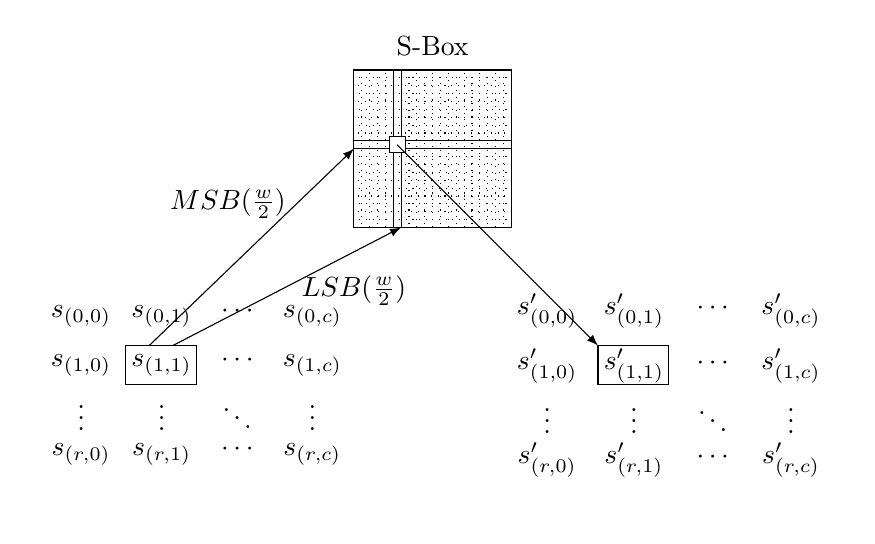
\begin{tikzpicture}[>=latex]

 \matrix (s) [matrix of math nodes,nodes = {node style ge},%
              %left delimiter  = (,right delimiter = ),
              column sep=-0.1cm,row sep=-0.5cm,
             ] at (-3,0)
        {
          s_{(0,0)} & s_{(0,1)} & \cdots & s_{(0,c)} \\
          s_{(1,0)} & s_{(1,1)} & \cdots & s_{(1,c)} \\
          \vdots    & \vdots    & \ddots & \vdots    \\
          s_{(r,0)} & s_{(r,1)} & \cdots & s_{(r,c)} \\
        };

\draw (-3.9,0.5)rectangle(-3,0);

 \matrix (s') [matrix of math nodes,nodes = {node style ge},%
              %left delimiter  = (,right delimiter = ),
              column sep=-0.1cm,row sep=-0.5cm,
             ] at (3,0)
        {
          s'_{(0,0)} & s'_{(0,1)} & \cdots & s'_{(0,c)} \\
          s'_{(1,0)} & s'_{(1,1)} & \cdots & s'_{(1,c)} \\
          \vdots    & \vdots    & \ddots & \vdots    \\
          s'_{(r,0)} & s'_{(r,1)} & \cdots & s'_{(r,c)} \\
        };
\draw (2.1,0.5)rectangle(3,0);

%sbox
\draw (-1,4)rectangle(1,2);
%x
\draw [dotted](-1,2.0)rectangle(1,2.1);
\draw [dotted](-1,2.2)rectangle(1,2.3);
\draw [dotted](-1,2.4)rectangle(1,2.5);
\draw [dotted](-1,2.6)rectangle(1,2.7);
\draw [dotted](-1,2.8)rectangle(1,2.9);
\draw (-1,3)rectangle(1,3.1);
\draw [dotted](-1,3.2)rectangle(1,3.3);
\draw [dotted](-1,3.4)rectangle(1,3.5);
\draw [dotted](-1,3.6)rectangle(1,3.7);
\draw [dotted](-1,3.8)rectangle(1,3.9);
%y
\draw [dotted](-.9,4)rectangle(-.8,2);
\draw [dotted](-.7,4)rectangle(-.6,2);
\draw (-.5,4)rectangle(-.4,2);
\draw [dotted](-.3,4)rectangle(-.2,2);
\draw [dotted](-.1,4)rectangle(0,2);
\draw [dotted](.1,4)rectangle(.2,2);
\draw [dotted](.3,4)rectangle(.4,2);
\draw [dotted](.5,4)rectangle(.6,2);fact
\draw [dotted](.7,4)rectangle(.8,2);
\draw [dotted](.9,4)rectangle(1,2);
%cell
\draw [fill=white] (-.55,2.95)rectangle(-.35,3.15);
%arrows
\draw [->] (-3.6,0.5)--(-1,3);%x
\draw [->] (-3.3,0.5)--(-.4,2);%y
\draw [->] (-.45,3.05)--(2.1,0.5);

%text
\node [rectangle] (sbox) at (0,4.3) {S-Box};
\node [rectangle] (msb) at (-2.6,2.3) {$MSB(\frac{w}{2})$};
\node [rectangle] (lsb) at (-1,1.2) {$LSB(\frac{w}{2})$};

\end{tikzpicture}
\caption{Schematic diagram of the subBytes() transformation}
\label{fig:subBytes}
\end{center}
\end{figure}

%%%%%%%%%%%%%%%%%%%%%%%%%%%%%%%%%%%%%%%%%%%%%%%%%%%%%%%%%%%%%%%%%%%%%%%%%%%%%%%
\subsubsection{How to build different SBoxes}\label{sec:sbox}

% and how to build a new one with different parameters
Using the same \emph{wordsize} there are two different things that can be changed: $b$ and $c$. The $c=$\texttt{0x63} and the product over the field of equation \ref{eq:subBytes:affine}. If the option is to use another wordsize this is the unique main parameter of the original Rijndael to set a different. With a wordsize of $4$ the operations will be defined over \Fpnm{4}{z}, over $16$ the field will be \Fpnm{{16}}{z}, and the subparameters of the affine transformation must also be set up.

\begin{itemize}
 \item \todo{how to build new $S$ and $S^{-1}$ for $w\neq 8$.}
 \begin{itemize}
  \item Why was chosen for $w=8 \Rightarrow m(z) = z^8+z^4+z^3+z+1$?
  \begin{itemize}
   \item Would be that \texttt{0b100011011} is the first (bigger than $z^8$) that has a Hamming weight of the half (by excess) of the length.
   \item \todo{If it's the case, reference to the Hamming weight definition \ref{def:hammingWeight}}
  \end{itemize}
  \item Irreducible polynomial with \emph{wordsize} degree, the firsts bigger than $x^w$ with a Hamming weight above the half of the length:
  \begin{itemize}
   \item $w=2 \rightarrow m(z) = z^2+z+1$: Non other below but bigger than $z^2$ is irreducible.
   \item $w=3 \rightarrow m(z) = z^3+z+1$: Hamming weight of \texttt{0b1011} is 3 (above 2).
   \item $w=4 \rightarrow m(z) = z^4+z+1$: Hamming weight of \texttt{0b10011} is 3 (above 3).
   %\item $w=4 \rightarrow m(z) = z^4+z^3+z^2+z+1$: Hamming weight of \texttt{0b11111} is 5 (above 3).
   \item $w=5 \rightarrow m(z) = z^5+z^2+1$: Hamming weight of \texttt{0b100101} is 3 (above 3).
   %\item $w=6 \rightarrow m(z) = z^6+z+1$: Hamming weight of \texttt{0b1000011} is 3 (below 4).
   %\item $w=6 \rightarrow m(z) = z^6+z^3+1$: Hamming weight of \texttt{0b1001001} is 3 (below 4).
   \item $w=6 \rightarrow m(z) = z^6+z^4+z^2+z+1$: Hamming weight of \texttt{0b1010111} is 5 (above 4).
   %\item $w=7 \rightarrow m(z) = z^7+z+1$: Hamming weight of \texttt{0b10000011} is 3 (below 4).
   %\item $w=7 \rightarrow m(z) = z^7+z^3+1$: Hamming weight of \texttt{0b10001001} is 3 (below 4).
   %\item $w=7 \rightarrow m(z) = z^7+z^4+1$: Hamming weight of \texttt{0b10010001} is 3 (below 4).
   \item $w=7 \rightarrow m(z) = z^7+z^4+z^3+z^2+1$: Hamming weight of \texttt{0b10011101} is 5 (above 4).
%   \item $w= \rightarrow m(z) = z^7$: Hamming weight of \texttt{0b1} is .
   \item \todo{Rule to chose the others, specially odds wordsizes but also bigger than $8$}.
  \end{itemize}
  \item build $g(z)$ in \Fpnm{w}{z}
  \item build $f(z)$ and $f^{-1}(z)$ in \Fpnm{w}{z}
  \begin{itemize}
   \item How to chose the circulant matrix from $b$ of equation \ref{eq:subBytes:affine} used in equation \ref{eq:subBytes:matrix} and the $c$ (and also for the inverse)?
  \end{itemize}
 \end{itemize}
 \item \todo{summarize the $S$ and $S^{-1}$ using $w=2$, $w=4$ and $w=16$ in their \emph{S-Box}es and their inverse Boxes.}
\end{itemize}


%%%%%%%%%%%%%%%%%%%%%%%%%%%%%%%%%%%%%%%%%%%%%%%%%%%%%%%%%%%%%%%%%%%%%%%%%%%%%%%
\subsection{shiftRows}\label{sec:shiftRows}
% abstraction of what it is, independent from the #rows, #columns, wordsize
Now we are over the second operation of a \emph{Rijndael} round --remember figure \ref{fig:RijndaelDiagram}--. This operation is a transposition, and again, in Shannon's terms this provides \emph{diffusion} to the schema. This operation takes the state matrix in rows to do a cyclic shift to the left over its cells, each row as many times as its index. Row $n$ cyclically shifted its cells $n$ times as the figure \ref{fig:shiftRows} represents for 4 rows --as the classic \emph{Rijndael} is--. As mention in \cite{Daemen:2002:DR:560131} (section 3.4.2) the assignment of number of offsets per rows is arbitrary, and they are done in this order for simplicity.

%\begin{itemize}
% \item \todo{What this means mathematically, independently to the parameters \#rows, \#columns, wordsize}
%\end{itemize}

% draw schematic of this step
\begin{figure}[h!]
\begin{center}
\def\origin{-3}
\def\dest{3}
\def\height{5}
\def\dist{1}

\tikzstyle{statecell}=[rectangle,
                                    thick,
                                    minimum size=1cm,
                                    draw=gray!80,
                                    fill=gray!20]

\tikzstyle{shiftedcell}=[rectangle,
                                    thick,
                                    minimum size=1cm,
                                    draw=gray!80,
                                    fill=red!20]

\begin{tikzpicture}[>=latex]


%input state matrix
\node (s00) at (\origin,\height) [statecell] {$\mathbf{s_{00}}$};
\node (s01) at (\origin+1*\dist,\height) [statecell] {$\mathbf{s_{01}}$};
\node (s02) at (\origin+2*\dist,\height) [statecell] {$\mathbf{s_{02}}$};
\node (s03) at (\origin+3*\dist,\height) [statecell] {$\mathbf{s_{03}}$};

\node (s10) at (\origin,\height-1*\dist) [statecell] {$\mathbf{s_{10}}$};
\node (s11) at (\origin+1*\dist,\height-1*\dist) [statecell] {$\mathbf{s_{11}}$};
\node (s12) at (\origin+2*\dist,\height-1*\dist) [statecell] {$\mathbf{s_{12}}$};
\node (s13) at (\origin+3*\dist,\height-1*\dist) [statecell] {$\mathbf{s_{13}}$};

\node (s20) at (\origin,\height-2*\dist) [statecell] {$\mathbf{s_{20}}$};
\node (s21) at (\origin+1*\dist,\height-2*\dist) [statecell] {$\mathbf{s_{21}}$};
\node (s22) at (\origin+2*\dist,\height-2*\dist) [statecell] {$\mathbf{s_{22}}$};
\node (s23) at (\origin+3*\dist,\height-2*\dist) [statecell] {$\mathbf{s_{23}}$};

\node (s30) at (\origin,\height-3*\dist) [statecell] {$\mathbf{s_{30}}$};
\node (s31) at (\origin+1*\dist,\height-3*\dist) [statecell] {$\mathbf{s_{31}}$};
\node (s32) at (\origin+2*\dist,\height-3*\dist) [statecell] {$\mathbf{s_{32}}$};
\node (s33) at (\origin+3*\dist,\height-3*\dist) [statecell] {$\mathbf{s_{33}}$};

%output state matrix
\node (s00_) at (\dest,\height) [statecell] {$\mathbf{s_{00}}$};
\node (s01_) at (\dest+1*\dist,\height) [statecell] {$\mathbf{s_{01}}$};
\node (s02_) at (\dest+2*\dist,\height) [statecell] {$\mathbf{s_{02}}$};
\node (s03_) at (\dest+3*\dist,\height) [statecell] {$\mathbf{s_{03}}$};

\node (s11_) at (\dest,\height-1*\dist) [statecell] {$\mathbf{s_{11}}$};
\node (s12_) at (\dest+1*\dist,\height-1*\dist) [statecell] {$\mathbf{s_{12}}$};
\node (s13_) at (\dest+2*\dist,\height-1*\dist) [statecell] {$\mathbf{s_{13}}$};
\node (s10_) at (\dest+3*\dist,\height-1*\dist) [shiftedcell] {$\mathbf{s_{10}}$};

\node (s22_) at (\dest,\height-2*\dist) [statecell] {$\mathbf{s_{22}}$};
\node (s23_) at (\dest+1*\dist,\height-2*\dist) [statecell] {$\mathbf{s_{23}}$};
\node (s20_) at (\dest+2*\dist,\height-2*\dist) [shiftedcell] {$\mathbf{s_{20}}$};
\node (s21_) at (\dest+3*\dist,\height-2*\dist) [shiftedcell] {$\mathbf{s_{21}}$};

\node (s33_) at (\dest,\height-3*\dist) [statecell] {$\mathbf{s_{33}}$};
\node (s30_) at (\dest+1*\dist,\height-3*\dist) [shiftedcell] {$\mathbf{s_{30}}$};
\node (s31_) at (\dest+2*\dist,\height-3*\dist) [shiftedcell] {$\mathbf{s_{31}}$};
\node (s32_) at (\dest+3*\dist,\height-3*\dist) [shiftedcell] {$\mathbf{s_{32}}$};

%arrows
\draw (s03) -- (s00_);
\draw[->] (s13) -- (s11_);
\draw[->>] (s23) -- (s22_);
\draw[->>] (s33) -- (s33_);
\end{tikzpicture}
\caption{Schematic diagram of the shiftRows() transformation \fixme{This diagram must be improved, use indexes on the cells} \fixme{rows $0$ is shifted $0$ cells (in standard but this is an arbitrary decision)}}
\label{fig:shiftRows}
\end{center}
\end{figure}

Its inverse operation is quite simple as the operation itself is, only that this time the cyclic shift is to the right the same number of times that was before to the left.

About the generalization of the \emph{Rijndael} schema, this operation does not show special hassles. There is only one restriction that makes a constrain in the generalization: there must not be two different rows that does the same number of shifts. And to complain that the number of rows must be equally or greater than the number or columns.

%%%%%%%%%%%%%%%%%%%%%%%%%%%%%%%%%%%%%%%%%%%%%%%%%%%%%%%%%%%%%%%%%%%%%%%%%%%%%%%
\subsection{mixColumns}\label{sec:mixColumns}
% abstraction of what it is, independent from the #rows, #columns, wordsize
This is the third operation of the \emph{Rijndael} round, and as it is a permutation in terms of Shannon this means that the step provides \emph{confusion} to the schema. In this case --and this is different than \emph{subBytes} from section \ref{sec:subBytes}-- this transformation is lineal.

This is the most complicated step in the \emph{Rijndael} under mathematical terms. This operation takes the columns of the states matrix and interprets it as elements in a polynomial ring. This mathematics has been introduced in section \ref{sec:math} with an example in \ref{sec:polynomialRing}. A columns represents an element of a polynomial ring $\frac{\Fpn{2}{w}[x]}{m'(x)}$ (with degree the number of rows: $deg(m')=\#rows$), where each of its cells are elements of a polynomial field $\Fpn{2}{w}=\frac{\mathbb{F}_{2}[z]}{m(z)}$  (with degree the word size: $deg(m)=wordsize$), and all the columns were operated with another element of the ring. This element, denoted by $c(x)$ in figure \ref{fig:mixColumns} must be invertible in the ring --remember that in a ring, not all the elements has inverse--.

% polynomial ring, where the coeficients are elements from a binary polynomial field
%   \Fpnm{x}{z}, deg(m)=#rows
%   (this is, imho, one of the most important points of rijndael)
% \begin{itemize}
%  \item \todo{What this means mathematically?} And what implies the changes on the parameters \#rows, \#columns, wordsize
%  \item \todo{polynomial ring} introduced in section \ref{sec:math}, where the coeficients are elements from a binary polynomial field \Fpnm{n}{x}, $deg(m)=\#rows$
% \end{itemize}

% FIXME (review) draw schematic of this step

\begin{figure}[h!]
\begin{center}
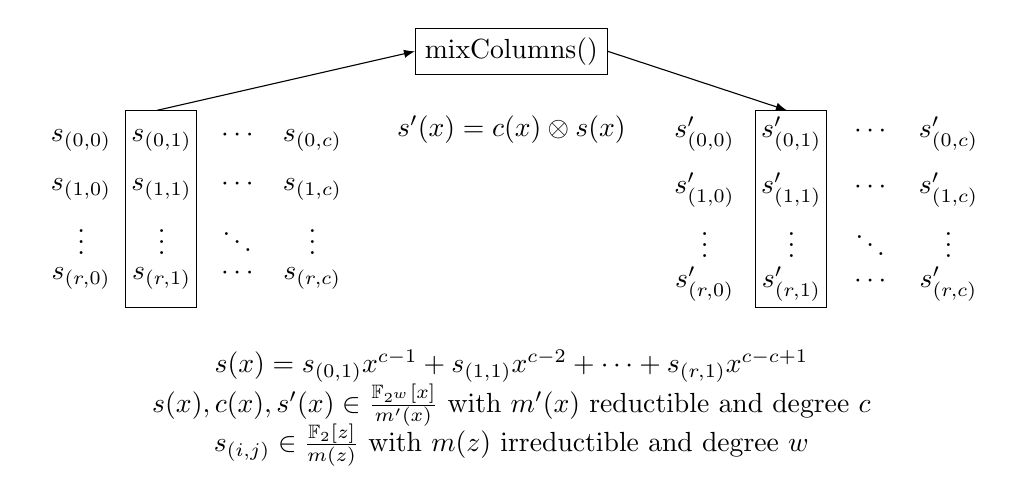
\begin{tikzpicture}[>=latex]
 
 \matrix (s) [matrix of math nodes,nodes = {node style ge},%
              %left delimiter  = (,right delimiter = ),
              column sep=-0.1cm,row sep=-0.5cm,
             ] at (-4,0)
        {
          s_{(0,0)} & s_{(0,1)} & \cdots & s_{(0,c)} \\
          s_{(1,0)} & s_{(1,1)} & \cdots & s_{(1,c)} \\
          \vdots    & \vdots    & \ddots & \vdots    \\
          s_{(r,0)} & s_{(r,1)} & \cdots & s_{(r,c)} \\
        };

\draw (-4.9,1.25)rectangle(-4,-1.25);

 \matrix (s') [matrix of math nodes,nodes = {node style ge},%
              %left delimiter  = (,right delimiter = ),
              column sep=-0.1cm,row sep=-0.5cm,
             ] at (4,0)
        {
          s'_{(0,0)} & s'_{(0,1)} & \cdots & s'_{(0,c)} \\
          s'_{(1,0)} & s'_{(1,1)} & \cdots & s'_{(1,c)} \\
          \vdots    & \vdots    & \ddots & \vdots    \\
          s'_{(r,0)} & s'_{(r,1)} & \cdots & s'_{(r,c)} \\
        };
\draw (3.1,1.25)rectangle(4,-1.25);

\node [rectangle,draw] (mixColumns) at (0,2) {mixColumns()};
 \draw [->] (-4.5,1.25)--(mixColumns.west);
 \draw [->] (mixColumns.east)--(3.5,1.25);

\node [rectangle] (poli) at (0,1.0) {$s'(x)=c(x)\otimes s(x)$};
\node [rectangle] (sx) at (0,-2) {$s(x)=s_{(0,1)}x^{c-1}+s_{(1,1)}x^{c-2}+\cdots+s_{(r,1)}x^{c-c+1}$};
\node [rectangle] (fpnm) at (0,-2.5) {$ s(x),c(x),s'(x) \in \frac{\Fpn{2}{w}[x]}{m'(x)}$ with $m'(x)$ reductible and degree $c$};
\node [rectangle] (fpn) at (0,-3) {$s_{(i,j)} \in \frac{\mathbb{F}_{2}[z]}{m(z)}$ with $m(z)$ irreductible and degree $w$};

\end{tikzpicture}
\caption{Diagram of the mixColumns() operation over the polynomial ring with coeficients in a polynomial field. Invert the mixColumns() is operate with $c^{-1}(x)=d(x)$ in the polynomial ring}
\label{fig:mixColumns}
\end{center}
\end{figure}

The inverse of this operation requires to inverse the polynomial $c(x)$ to do the same operation in the polynomial ring to reverse the column on the state matrix.

%%%%%%%%%%%%%%%%%%%%%%%%%%%%%%%%%%%%%%%%%%%%%%%%%%%%%%%%%%%%%%%%%%%%%%%%%%%%%%%
\subsection{Speeding the polynomial ring product operation}\label{sec:improvePolynomialRingProduct}
In section \ref{sec:polynomialRing} the operation between elements of this kind of polynomial ring that has coefficients in a binary polynomial field, has been explained. But there is an specific improvement of the \emph{product} operation that gives a valuable advantage to speed up this step of the process. 

In the specification of the rijndael schema \cite{Daemen01aes-ammended} is proposed the use of a circulant invertible matrix. In the \emph{mixColumns} operation, is set one fix element of the ring to be operated with each of the columns of the state matrix (in the interpretation of the column where each cell is one coefficient of this polynomial).

Then the fix polynomial element in the ring have set in the standard:
$$c(x) = (z+1)x^3+(1)x^2+(1)x+(z)$$
This is using the best notation to denote that the coefficients on the polynomial ring are elements of a polynomial field. The polynomial field have binary coefficients, then those polynomials can be shorted using a binary notation. Like $(z+1)=\texttt{0b11}=\texttt{0x3}$ and other like $(z^3+z+1)=\texttt{0b1011}=\texttt{0xB}$. Then this $c(x)$ can be shorted represented by: $c(x) = \texttt{0x3}x^3+\texttt{0x1}x^2+\texttt{0x1}x+\texttt{0x2}$. This polynomial element is coprime to the modulo ($x^4+1$) and therefore has an inverse in the ring used to revert the \emph{mixColumns}: $c^{-1}(x) = \texttt{0xB}x^3+\texttt{0xD}x^2+\texttt{0x9}x+\texttt{0xE}=d(x)$.

The matrix multiplication of this polynomial ring operation can be written as:
\begin{equation}\label{eq:MDS}
  \begin{bmatrix}
    s'_{(0,i)}\\s'_{(1,i)}\\s'_{(2,i)}\\s'_{(3,i)}
  \end{bmatrix}
  =
  \begin{bmatrix}
    z & z+1 & 1 & 1 \\
    1 & z & z+1 & 1 \\
    1 & 1 & z & z+1 \\
    z+1 & 1 & 1 & z \\
  \end{bmatrix}
  \begin{bmatrix}
    s_{(0,i)}\\s_{(1,i)}\\s_{(2,i)}\\s_{(3,i)}
  \end{bmatrix}
\end{equation}

\begin{itemize}
 \item \todo{What's a MaxDistanceSeparable Matrix?}
 \item \todo{Does this circulant matrix works with $c\neq 4$?}
\end{itemize}

%%%%%%%%%%%%%%%%%%%%%%%%%%%%%%%%%%%%%%%%%%%%%%%%%%%%%%%%%%%%%%%%%%%%%%%%%%%%%%%
\subsubsection{mixColumns with different number of rows}

\begin{itemize}
 \item \todo{Different number of rows means different degree on the polynomial ring than a column means}
 \item \todo{How to find a composited polynomial of the wanted degree? How to rule this to have it standardised and no need to deal with it to advice on the decryption}
 \item \todo{How to find an invertible element $c(x)$? How to standardised to avoid extra information requirement to the decipher?}
\end{itemize}

%%%%%%%%%%%%%%%%%%%%%%%%%%%%%%%%%%%%%%%%%%%%%%%%%%%%%%%%%%%%%%%%%%%%%%%%%%%%%%%
\subsection{addRoundKey}\label{sec:addRoundKey}

Even this is the first operation in in the \emph{Rijndael} schema (review figure \ref{fig:RijndaelDiagram}), it is considered the last of the four of one round. This operation is a substitution of the elements in the cells of the state matrix, and because of that, on the Shannon's view this provides \emph{confusion} to the schema. This is the only operation in the \emph{Rijndael} that interacts with the expanded key, and the operation is a \emph{bitwise xor}, the addition of the very basic bricks below \emph{Rijndael} maths, the binary field $\mathbb{F}_{2}$.

\begin{itemize}
 %\item \todo{this is the operation where the key is used (from the 4 rijndael operations)}
 %\item \todo{simply a xor operation (addition in \Fq{2})}
 \item \todo{Explain why the state matrix is taken by columns if the \emph{xor} is for bit elements? It's nothing more than simplicity with the common 32 bit architecture}
\end{itemize}

\begin{figure}[h!]
\begin{center}
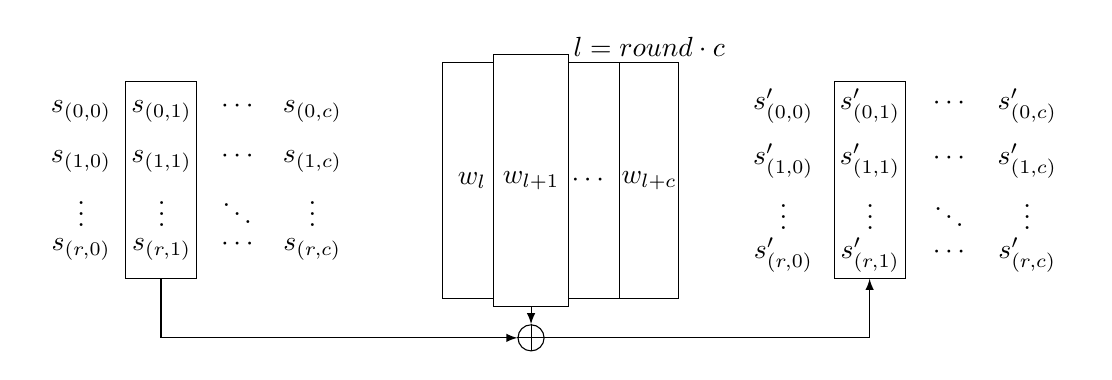
\begin{tikzpicture}[>=latex]
 
\matrix (s) [matrix of math nodes,nodes = {node style ge},%
              %left delimiter  = (,right delimiter = ),
              column sep=-0.1cm,row sep=-0.5cm,
             ] at (-5,0)
        {
          s_{(0,0)} & s_{(0,1)} & \cdots & s_{(0,c)} \\
          s_{(1,0)} & s_{(1,1)} & \cdots & s_{(1,c)} \\
          \vdots    & \vdots    & \ddots & \vdots    \\
          s_{(r,0)} & s_{(r,1)} & \cdots & s_{(r,c)} \\
        };

\draw (-5.9,1.25)rectangle(-5,-1.25);

 \matrix (s') [matrix of math nodes,nodes = {node style ge},%
              %left delimiter  = (,right delimiter = ),
              column sep=-0.1cm,row sep=-0.5cm,
             ] at (4,0)
        {
          s'_{(0,0)} & s'_{(0,1)} & \cdots & s'_{(0,c)} \\
          s'_{(1,0)} & s'_{(1,1)} & \cdots & s'_{(1,c)} \\
          \vdots    & \vdots    & \ddots & \vdots    \\
          s'_{(r,0)} & s'_{(r,1)} & \cdots & s'_{(r,c)} \\
        };
\draw (3.1,1.25)rectangle(4,-1.25);
%the central boxes of the key table
\draw        (-1.875,1.5)rectangle(-1.125,-1.5);\node [] (wl) at (-1.5,0) {$w_{l}$};
\draw        (-0.375,1.5)rectangle( 0.375,-1.5);\node [] (wld) at (0,0) {$\cdots$};
\draw        ( 0.375,1.5)rectangle( 1.125,-1.5);\node [] (wlc) at (.75,0) {$w_{l+c}$};
%the bigger column
\draw [fill=white] (-1.225,1.6)rectangle(-0.275,-1.6);\node [] (wl1) at (-.75,0) {$w_{l+1}$};
%the xor sign
\node [circle,draw] (xor) at (-.75,-2) {};
 \draw [-] (xor.north) -- (xor.south);
 \draw [-] (xor.west) -- (xor.east);
%algorithm lines
\draw [->] (-5.45,-1.25)--(-5.45,-2)--(xor.west);
\draw [->] (-.75,-1.6)--(xor.north);
\draw [->] (xor.east)--(3.55,-2)--(3.55,-1.25);

\node [] (l) at (0.75,1.7) {$l=round\cdot c$};

\end{tikzpicture}
\caption{Diagram of the addRoundKey()}
\label{fig:addRoundKey}
\end{center}
\end{figure}


%%%%%%%%%%%%%%%%%%%%%%%%%%%%%%%%%%%%%%%%%%%%%%%%%%%%%%%%%%%%%%%%%%%%%%%%%%%%%%%
\section{Parameter combinations}\label{sec:parameterCombinations}
%how, with different parameters, can have the same block sizes, and what's different between them
\begin{itemize}
 \item \todo{different parameter combinations} can produce the same block (and key) sizes. What can help on the option chose?
 \item \todo{Remember, from \emph{shiftRows} section \ref{sec:shiftRows}, the number of rows must be equal or greater than number of columns.}
 \item \todo{Can the wordsize be smaller than \#rows? It looks that no restriction in this. There is no relation between the degree of the elements in of the polynomial ring $\frac{\Fpn{2}{w}[x]}{m'(x)}$, with the degree of the coefficients that are elements on a polynomial field $\frac{\Fpn{2}[z]}{m(z)}$}
\end{itemize}


%%%%%%%%%%%%%%%%%%%%%%%%%%%%%%%%%%%%%%%%%%%%%%%%%%%%%%%%%%%%%%%%%%%%%%%%%%%%%%%
\section{New useful sizes for Rijndael}\label{sec:newSizes}
% because of the newer processors with 64 bits, it can be easy to have bigger sizes with less costs
\begin{itemize}
 \item \todo{With the newer architectures (64bits) which parameter changes can improve the cost of the rijndael?} \cite{Daemen:1999:EBC:1267115.1267119}
 \item Small sizes of \emph{Rijndael} vs. lightweight alternatives (like \emph{Present}: $64b$ block with keys between $80b$ and $128b$.
 \item Check the AES contest tests with those new sizes
\end{itemize}

%%%%%%%%%%%%%%%%%%%%%%%%%%%%%%%%%%%%%%%%%%%%%%%%%%%%%%%%%%%%%%%%%%%%%%%%%%%%%%%
% what else would be in this paper?
\section{Attacking the schema}\label{sec:attacks}

\todo{Who the current attacks affects this variations on the possible sizing?}

\subsection{Side channel attacks}\label{sec:sideChannel}
\begin{itemize}
\item \todo{differences between precalculated sbox and rcon or better to compute on the fly?}\\
\item \todo{constant time operation intervals and equivalent memory use}\\
\item \todo{key expansion calculated during the encrypt/decrypt process}
\end{itemize}

\section{New sizes with in the AESWrap \cite{rfc3394}}\label{sec:aeswrap}
\todo{}

\section{Conclusions}\label{sec:conclusion}
\todo{}

%%%%%%%%%%%%%%%%%%%%%%%%%%%%%%%%%%%%%%%%%%%%%%%%%%%%%%%%%%%%%%%%%%%%%%%%%%%%%%%
\bibliographystyle{ieeetr}
\bibliography{../bibtex/sblanch.bib,../bibtex/rijndael.bib,../bibtex/symmetrics.bib,../bibtex/standards.bib,../bibtex/books.bib,../bibtex/crypto.bib,../bibtex/rfc.bib}

\end{document}